\PassOptionsToPackage{unicode,pdfusetitle}{hyperref}
\PassOptionsToPackage{hyphens}{url}

\documentclass[twoside]{article}
\usepackage[a4paper,includeheadfoot,top=0cm,bottom=0.2cm,left=1.5cm,right=0.2cm]{geometry}
\usepackage{amsmath,amssymb}
\usepackage{fontspec}
\usepackage[russian]{babel}
\usepackage{microtype}
\usepackage{parskip}
\usepackage{xcolor}
\definecolor{navy}{RGB}{0,0,128}
\setmainfont{Noto Serif}
\setsansfont{Monitorica}
\setmonofont{Noto Sans Mono}
\newfontfamily\headingfont{Operation Napalm}
\usepackage{titlesec}
\titleformat{\section}{\headingfont\color{navy}\Large}{\thesection}{1em}{}[\titlerule]
\titleformat{\subsection}{\headingfont\color{navy}\large}{\thesubsection}{1em}{}
\titleformat{\subsubsection}{\headingfont\color{navy}\normalsize}{\thesubsubsection}{1em}{}
\titleformat{\paragraph}{\headingfont\color{navy}\normalsize}{\theparagraph}{1em}{}
\titleformat{\subparagraph}{\headingfont\color{navy}\normalsize\itshape}{\thesubparagraph}{1em}{}
\usepackage{multicol}
\usepackage{array}
\usepackage{background}
\usepackage{wallpaper}
\usepackage{tabularray}
\usepackage{tblr-extras}
\usepackage{multirow}
\usepackage{makecell}
\usepackage{calc}
\usepackage{rotating}
\usepackage{caption}
\usepackage{capt-of}
\usepackage{titletoc}
\usepackage{graphicx}
\UseTblrLibrary{booktabs,caption,babel}
\makeatletter
\def\maxwidth{\ifdim\Gin@nat@width>\linewidth\linewidth\else\Gin@nat@width\fi}
\def\maxheight{\ifdim\Gin@nat@height>\textheight\textheight\else\Gin@nat@height\fi}
\makeatother
% Set default figure placement to htbp
\makeatletter
\def\fps@figure{htbp}
\makeatother
\setlength{\emergencystretch}{3em}
\providecommand{\tightlist}{
  \setlength{\itemsep}{0pt}\setlength{\parskip}{0pt}}
\setcounter{secnumdepth}{5}
\setcounter{tocdepth}{5}
\titlecontents{section}[0em]{}{\headingfont\Large\makebox[1.3em][l]{\thecontentslabel}}{}{\titlerule*[0.8pc]{.}\contentspage}
\titlecontents{subsection}[0em]{}{\headingfont\large\makebox[2.1em][l]{\thecontentslabel}}{}{\titlerule*[0.8pc]{.}\contentspage}
\titlecontents{subsubsection}[0em]{}{\headingfont\makebox[3.2em][l]{\thecontentslabel}}{}{\titlerule*[0.8pc]{.}\contentspage}
\titlecontents{paragraph}[0em]{}{\headingfont\small\makebox[4.2em][l]{\thecontentslabel}}{}{\titlerule*[0.8pc]{.}\contentspage}
\titlecontents{subparagraph}[0em]{}{\headingfont\footnotesize\makebox[5.0em][l]{\thecontentslabel}}{}{\titlerule*[0.8pc]{.}\contentspage}
\usepackage{bookmark}
\IfFileExists{xurl.sty}{\usepackage{xurl}}{} % add URL line breaks if available
\urlstyle{same}
\hypersetup{
  hidelinks
}

\captionsetup{labelfont={it,color=navy},textfont={it,color=navy},justification=centering}
\captionsetup[table]{hypcap=false}
\captionsetup[figure]{hypcap=false}
\addto\extrasrussian{
  \def\figurename{Схема}
  \def\tableautorefname{Таблица}
  \def\figureautorefname{Схема}
  \def\sectionautorefname{Раздел}
  \def\subsectionautorefname{Подраздел}
  \def\subsubsectionautorefname{Параграф}
  \def\paragraphautorefname{Абзац}
  \def\pageautorefname{Страница}
  \def\equationautorefname{Формула}
}

\title{Контракт}
\newcommand{\siteurl}{https://vk.com/playingwar}
\author{Никита Макаров}

\begin{document}

\begin{titlepage}
\backgroundsetup{
  scale=1,
  angle=0,
  opacity=1,
  position={current page.center},
  contents={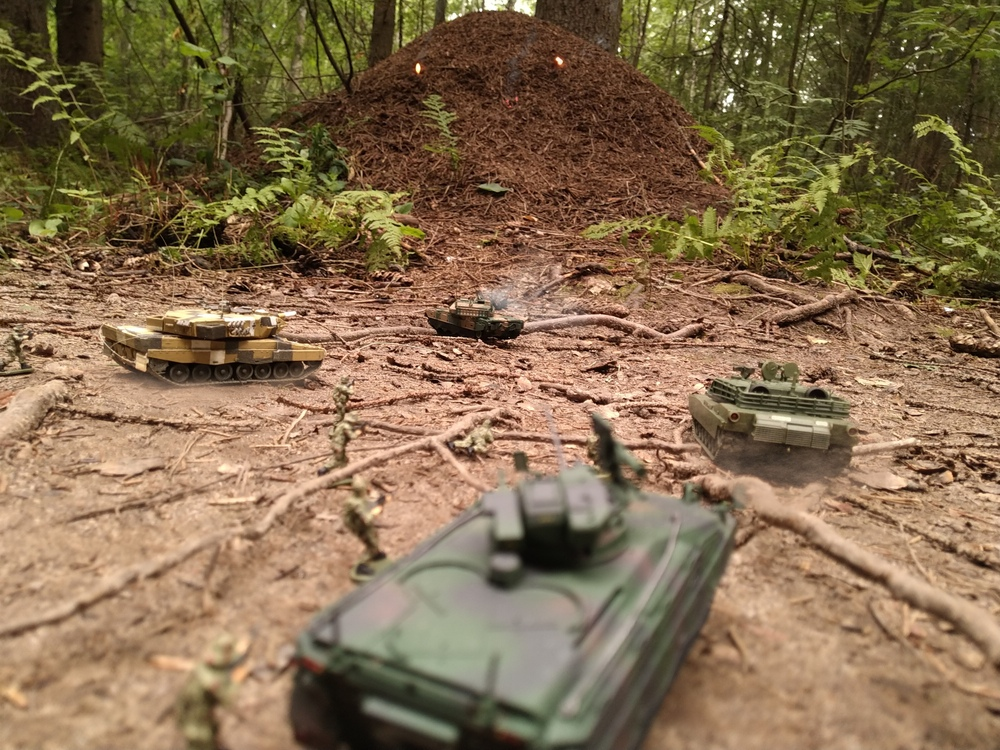
\includegraphics[width=\paperwidth*2,height=\paperheight,clip]{media/contract/image2.jpg}}
}

\begin{center}
\vspace*{2cm}

{\color{white}\headingfont\fontsize{48}{56}\selectfont{Контракт}}

\vspace{0.5cm}

{\color{white}\headingfont\fontsize{32}{40}\selectfont{Ролевая тактическая игра}}

%\maketitle

\vfill

{\color{white}\Large\textbf{Никита Макаров}}

{\color{white}\href{\siteurl}{\textbf{\MakeUppercase{\siteurl}}}}

{\color{white}\textbf{Санкт-Петербург}}

\end{center}
\end{titlepage}

\clearpage

\backgroundsetup{
  scale=1,
  angle=0,
  opacity=1,
  position={current page.center},
  contents={\TileWallPaper{1cm}{1cm}{media/common/image1.jpg}}
}

\begin{multicols}{2}
\raggedcolumns{}

\renewcommand{\contentsname}{Содержание}
\tableofcontents
\thispagestyle{empty}
\BgThispage{}

\clearpage

\section{Об игре}\label{intro}

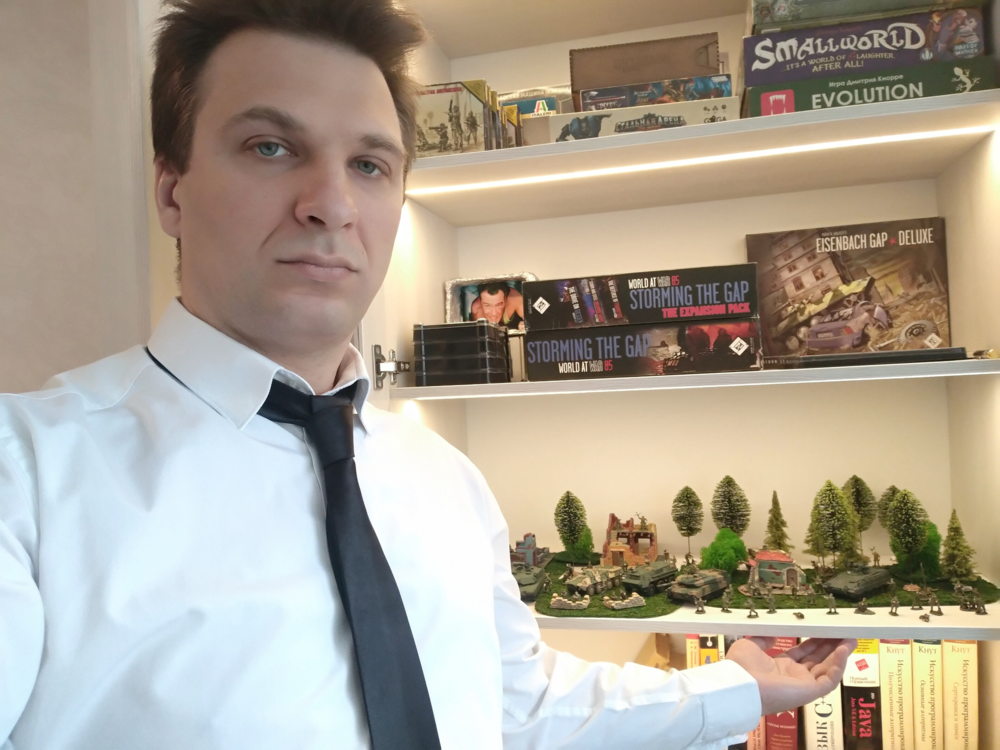
\includegraphics[width=\linewidth]{media/contract/image3.png}

Когда-то в детстве автор любил играть с кубиками и строить города.
Однажды он нашёл миниатюрных солдатиков. Что с ними делать?
Автор не знал. Взрослые рассказали ему, что есть специальные правила, с помощью которых можно организовывать
сражения. Кто же будет соперником автора в этих сражениях?

На юность автора пришёлся рассвет эры персональных компьютеров и компьютерных игр,
в том числе стратегий. Компьютер стал играть роль и соперника, и посредника. Однако,
автор ценит человеческое общение и любит встретиться с соперником лицом к лицу.

Автор написал небольшую книжку под названием ``Истории о военных играх'', во время работы
над которой познакомившись с трудами Герберта Уэллса, Джеймса Даннигана, Марка
Германа, Константина Кривенко и Рори Крэбба и изучив историю военных игр и их ключевые особенности.

Вдохновляясь этими людьми и такими их творениями как Art of Tactic,
Fireteam: Modern и Team Yankee, была спроектирована основа симуляции
боя, основным отличием которой считалось сочетание высокой динамичности
и простоты. Выражалось это, в основном, в переходе на \textbf{разрешение всех
задач броском одной двадцатигранной игральной кости D20} с использованием
таблиц эффектов в случаях, когда необходимо неравномерное (например, нормальное)
распределение вероятностей.

Далее симуляция развивалась под впечатлением от книги Modern War in
Miniature 1966 года за авторством Майкла Корнса, который позднее работал
в главном центре военных игр армии США, расположенном в Форт Ливенворте,
и занимался исследованием психологии на поле боя, вводя в военные игры
статистические модели психоэмоциональной устойчивости солдат.

Наконец, автор понял, что ему не хватает смысла, стоящего за механикой
симуляции, и начал искать способы глубже погрузиться в игру и
моделировать более комплексные взаимодействия персонажей, рассматривая
такие примеры как Dungeons and Dragons, GURPS, Only War от компании FFG,
Modern War от Zozer.

Симуляция была провалидирована с использованием документации United
States Army Field Manuals, в том числе с использованием LLM, а также
протестирована в игре с реальными людьми.

Из опыта общения с игроками в настольные ролевые игры автор знает, что для многих игроков броски кубиков --- это важная
часть процесса игры, фактически игра в игре, однако сам воспринимает их
всего лишь как один из способов получить случайное число и предпочитает
вместо реальных кубиков использовать цифровое приложение, например, RPG Simple Dice для Android.

Автор разработал собственное веб-приложение, реализующее большинство аспектов и механик данных правил для облегчения и ускорения игры, автоматизации рутинных действий.
С помощью этого приложения играть можно вообще без кубиков и стола, но для любителей кубиков
есть возможность вводить выпавшие значения в приложение. Мастер игры, выступая посредником между
игроками, может создавать для игроков ``туман войны'': не выставлять на игровое поле фигурки,
которые в настоящее время не видны персонажам игроков. Для этого ему нужно было бы иметь
отдельное поле, где можно было бы отслеживать позиции всех отрядов. Приложение может выступать
таким полем, поскольку оно содержит интерактивную схему. Кроме того, оно позволят печатать листы отрядов.

\begin{center}
https://github.com/guidebot/peace\_and\_prosperity
\end{center}

\section{Масштаб и период}\label{scale-period}

Автор поставил перед собой амбициозную задачу показать каждого персонажа
крупным планом, и при этом дать им всем возможность поучаствовать в
довольно масштабных военизированных операциях, включающих десятки
человек, использующих современное дальнобойное вооружение. Каждый игрок
имеет персонификацию в игровом мире, но контролирует не просто своего персонажа,
а целый отряд, а может быть, и не один.

Симуляция обеспечивает воспроизведение боёв сухопутных войск
численностью уровня до роты с детализацией уровня отдельных солдат и
единиц техники. Игрок обычно управляет эквивалентом взвода.
Предусмотрены такие виды техники как танки, БМП, ПТРК,
разведывательные и ударные дроны разных типов, миномёты, артиллерия,
средства связи и радиоэлектронной борьбы.

\textbf{Наименьший отрезок времени в бою (ход) соответствует 30 секундам.
Пространственный масштаб 1/1000, то есть 1 см соответствует 10 м.}

Автор рекомендует не воспринимать эти цифры слишком буквально, не
вымерять миллиметры, и даже допускает измерения «на глаз». По его
мнению, плюс/минус один сантиметр в этой игре решающего значения не
имеет.

Боевые единицы могут быть представлены плоскими квадратными фишками с
длиной стороны 1 см, а элементы локации --- листами бумаги различной
формы, что, по мнению автора, хорошо подойдёт к пространственному
масштабу игры.

\subsection{Использование миниатюр}\label{miniatures}

Автор признаёт, что красивые покрашенные миниатюры могут доставить
значительное эстетическое удовольствие и повысить вовлечённость в игру.
Автор и сам практикует использование фигурок масштаба 1/100 или даже
1/72. Однако, вынужден предупредить, что при использовании фигурок
придётся смириться с тем, что визуализация будет не вполне
соответствовать системному масштабу игры, и из-за этого подчас можно
почувствовать некоторый диссонанс. Здесь выбор остаётся за игроками, но
автор позволит себе дать несколько советов для тех, кто будет
организовывать игру с миниатюрами. Важно помнить, что фигурки и фишки не
обязательно отражают реальные габариты, это просто маркеры, а реальные
боевые единицы находятся где-то в их пределах, но занимают гораздо
меньшую площадь.

Итак, при игре миниатюрами предполагается, что элементы локации (здания,
деревья и так далее) будут соответствующего масштаба. Автору нравится
использовать листы натурального мха для представления лесных зон, на
которые выставляется несколько моделей деревьев, которые символически
отображают принадлежность полигона к лесной зоне, и при этом могут быть
легко перемещены внутри этой зоны для удобства измерения расстояний или
размещения миниатюр персонажей.

При использовании миниатюр в масштабе 1/72 модель дома может быть
размером 10×10 см. В масштабе игры это будет огромное здание размером
100×100 м, целый торговый центр, хотя визуально это будет изба 10×10 м.
При высоте фигурки человека 2--2,5 см, дистанция броска гранаты в 4 см
может выглядеть странно.

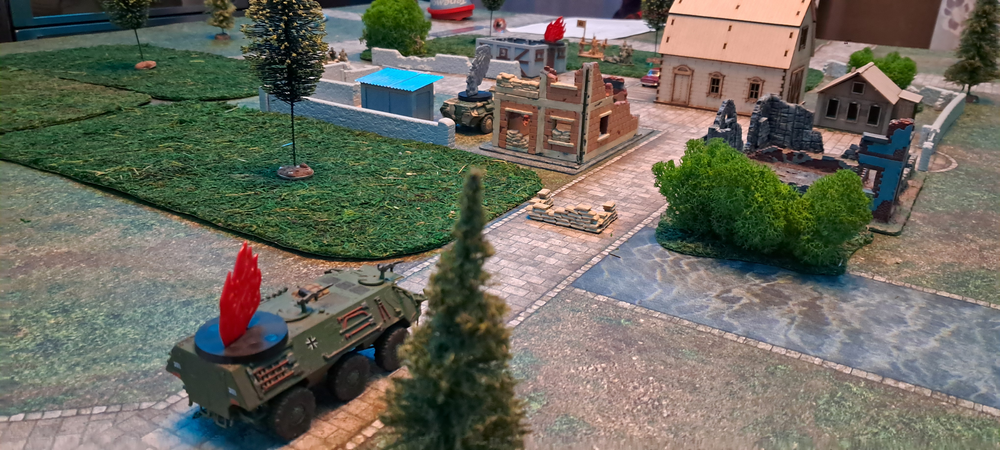
\includegraphics[width=\linewidth]{media/contract/image4.png}

Чтобы уменьшить визуальный диссонанс, автор
предлагает использовать так называемый \textbf{метод неравномерного
пространства}. Дистанции переводятся из реального масштаба в игровой не
по формуле см~=~м~×~0.1, а по формуле см~=~м~×~0.1~+~x, где x --- это
некоторая константа, в качестве которой рекомендуется выбрать число в
диапазоне 4--9 (автор использует 4). Также и при переводе из игрового масштаба в реальный
используется не м~=~см~×~10, а м~=~(см~--~x)~×~10 (естественно, это
число не имеет смысла, когда оно отрицательно). Таким образом вокруг
каждого отряда образуется пятно радиусом x~+~1~см, которое соответствует
10 м реального масштаба, но каждый 1~см сверх этого радиуса прибавляет
ещё 10~м к дистанции. Например, при x~=~9: 10~см соответствует 10~м,
11~см соответствует 20~м, 12~см соответствует 30~м и так далее. Эти
формулы применяются только к расчётам дистанций для применения оружия и
экипировки, в том числе наблюдения. Передвижение осуществляется обычно.

При использовании зданий метод неравномерного пространства имеет
особенности. Для уменьшения диссонанса внутри здания расстояния можно не
измерять. Вместо этого можно разделить здание на сектора, перекрывающие
линии видимости и огня (помещения). Отряд пехоты в помещении может
свободно перемещаться по нему; линии видимости и огня вовне помещения
проводятся от края помещения, при этом они не учитывают конфигурацию
окон и дверей --- если в стене помещения есть дверь или окно, считается,
что это окно во всю стену; при входе и выходе из здания расстояние
измеряется также от края помещения.

\section{Основы}\label{basics}

\subsection{Атрибуты и навыки персонажей}\label{attributes}

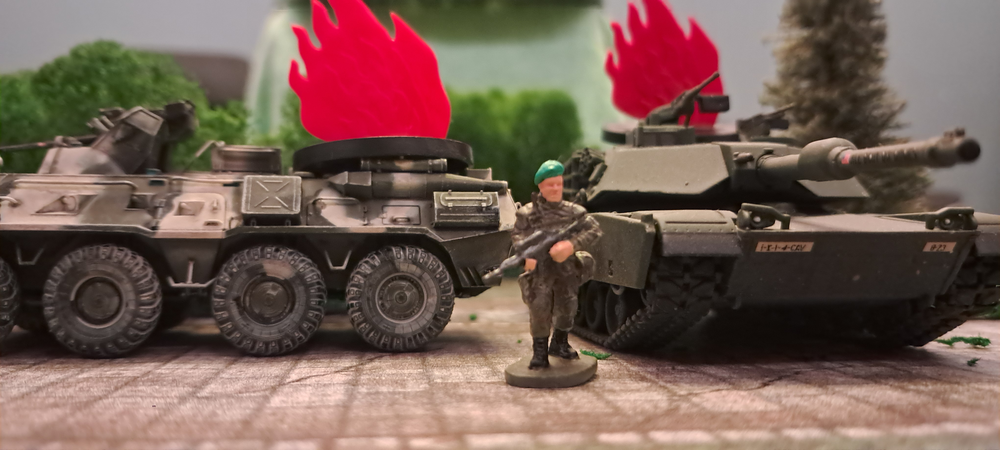
\includegraphics[width=\linewidth]{media/contract/image5.png}

Как и во многих других системах ролевых игр, у персонажей есть наборы
атрибутов и навыков. Навыки привязаны к одному из атрибутов.

Значения атрибутов используются для ограничения максимального значения
соответствующих навыков. Допускается игра без указания атрибутов, тогда
\textbf{персонажи могут развивать все навыки до максимума --- 20 очков
тренированности}.

Навыки персонажа определяют его эффективность в различных ситуациях и
являются результатом интенсивных тренировок либо боевого опыта. Однако,
навыки могут ухудшаться из-за травм или редкого применения, а чтобы
стать в чём-то экспертом требуются серьёзные усилия. Каждое очко
тренированности --- это 28 часов интенсивных тренировок.

Для определения эффективности солдата в различных ситуациях могут
использоваться как сами очки тренированности, так и уровень навыка,
который напрямую зависит от тренированности и обозначается как Ур(х),
где х --- очки тренированности в некотором навыке. Уровень позволяет перейти
от равномерной шкалы к более реальному распределению.

\begin{minipage}{\columnwidth}
\small
\begin{talltblr}[
  caption = {Атрибуты и навыки},
  label = {table-attributes}
]{
  hlines,
  row{odd}={fg=navy},
  row{even}={fg=black},
  colspec={Q[l,m,co=2]Q[c,m,co=4]Q[r,m,co=1]}
}
\SetCell{c,m} Атрибут & \SetCell[c=2]{c,m} Навыки \\
Здоровье & Выносливость & ВНС \\
\SetCell[r=2]{l,m} Ловкость & Маневрирование & МНВ \\
& Маскировка & МСК \\
\SetCell[r=7]{l,m} Меткость & Метательное оружие (гранаты) & ГРН \\
& Лёгкое стрелковое оружие & ЛС \\
& Снайперское оружие & СН \\
& Пулемёты & ПЛМ \\
& Управляемые ракеты & УР \\
& Управляемые дроны & ДРН \\
& Тяжёлое вооружение & ТВ \\
Интеллект & Медицина & МЕД \\
& Механика & МЕХ \\
& Электроника & ЭЛ \\
& Взрывчатые вещества & ВЗР \\
& Огневая поддержка & ОП \\
& Логика & ЛГК \\
Харизма & Влияние & ВЛН \\
\end{talltblr}
\end{minipage}

Навыки ЛГК и ВЛН используются при определении порядка действия отрядов и
при восстановлении эффективности отряда после полученного
стресса\footnote{См. стр.~\pageref{action-phase}, \ref{action-phase}~\nameref{action-phase}.}. При этом выбирается
наибольшее значение из этих двух навыков. Далее в тексте это
обозначается как Макс(ЛГК/ВЛН).

\begin{center}
\begin{minipage}{0.6\columnwidth}
\small
\begin{talltblr}[
  caption = {Очки тренированности и навыка},
  label = {table-skill-levels}
]{
  hlines,
  row{odd}={fg=navy},
  row{even}={fg=black},
  colspec={Q[c,m,co=1]Q[c,m,co=1]},
}
Очки тренированности х & Уровень навыка Ур(x) \\
1--2 & 1 \\
3--6 & 2 \\
7--11 & 3 \\
12--15 & 4 \\
16--19 & 5 \\
20 & 6 \\
\end{talltblr}
\end{minipage}
\end{center}

\subsubsection{Выносливость (ВНС)}\label{endurance}

Навык определяет максимальный вес, который солдат может нести, скорость
передвижения и возможность преодоления препятствий. В ролевой части
навык ВНС используется в ситуациях, связанных с применением силы, в том числе в драках.

Обычный здоровый, но не спортивный человек получает 5 ВНС. Человек, регулярно занимающийся спортом 9 ВНС.

Грузоподъёмность персонажа определяется как $12 × Ур(ВНС) кг$.

При $ВНС = 0$ грузоподъёмность равна 0, это означает серьёзную болезнь и инвалидность персонажа, фактически, полную недееспособность.

Максимальная грузоподъёмность отряда складывается из грузоподъёмности каждого персонажа в отряде. Таким образом отряд из нескольких человек
может переносить тяжёлые вещи, например, миномёт с боезапасом.

Скорость пешего передвижения отряда при ненулевой грузоподъёмности определяется пропроционально текущей нагрузке.

\begin{minipage}{\columnwidth}
\begin{talltblr}[
  caption = {Скорость пешего передвижения в зависимости от нагрузки},
  label = {table-movement}
]{
  hlines,
  row{odd}={fg=navy},
  row{even}={fg=black},
  colspec={Q[c,m,co=3]Q[c,m,co=3]Q[c,m,co=1]}
}
\SetRow{font=\footnotesize}Нагрузка в \% от макс. грузоподъёмности & Скорость пешего передвижения, см & Бег \\
0\%--25\% & 5 & $+$ \\
25\%--50\% & 4 & $+$ \\
50\%--75\% & 3 & $+$ \\
75\%--100\% & 2 & $-$ \\
\end{talltblr}
\end{minipage}

При нагрузке менее 75\% отряд может двигаться бегом со скоростью в два раза выше пешей скорости.
При передвижении бегом отряд должен получить очко усталости\footnote{См. стр. \pageref{fatigue}, \ref{fatigue} \nameref{fatigue}.}.
Очков усталости у отряда не может быть больше, чем минимальный Ур(ВНС) среди персонажей отряда.

\paragraph{Пример}\label{example-endurance}

Отряд из 3 человек с ВНС~=~3 (Ур(ВНС)~=~2) у каждого может нести
снаряжение общим весом не более 72 кг. Если такой отряд несёт только 3
штурмовые винтовки (каждая весом 4,7 кг c боезапасом), то у него 14,1 кг
нагрузки, что составляет менее 20\%. Такой отряд может идти со скоростью
5 см за ход или бежать на 10 см за ход.

Если этот отряд возьмёт ручной противотанковый гранатомёт с боезапасом
общим весом 12,3 кг, то его нагрузка будет 26,4 кг, что составляет около
37\%, в результате чего он будет двигаться пешком со скоростью 4 см за ход
или бегом со скоростью 8 см за ход.

Если этот отряд возьмёт ещё ПТРК Фагот с двумя ракетами общим весом 44
кг, то нагрузка станет около 98\%, его скорость будет уже всего 2 см за
ход и он не сможет двигаться бегом.

\subsubsection{Маневрирование (МНВ)}\label{maneuver}

Навык определяет отработанные до автоматизма привычки, уменьшающие площадь поражения тела до минимума.
Человек умеет двигаться так, чтобы свести к минимуму риск попадания под обстрел, постоянно оценивает местность
и держит в голове ближайшие естественные укрытия, своевременно и оптимально меняет позы.

Высокий уровень навыка уменьшает вероятность поражения при стрельбе по отряду.

При определении навыка маневрирования Ур(МНВ) отряда среди солдат отряда выбирается минимальное значение
\footnote{См. стр. \pageref{mod-skill}, \ref{mod-skill} \nameref{mod-skill}.}.

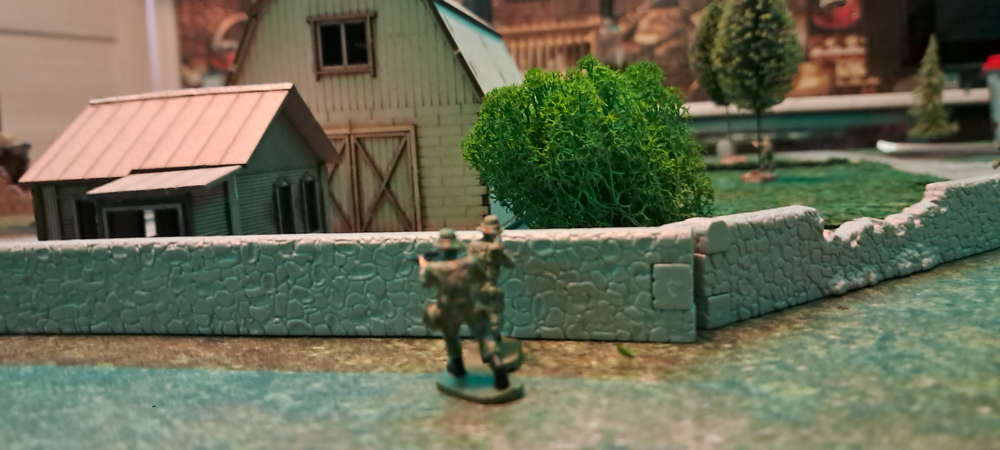
\includegraphics[width=\linewidth]{media/contract/image6.png}

\subsubsection{Маскировка (МСК)}\label{camouflage-skill}

Тренировки по маскировке включают в себя собственно маскировку\footnote{См. стр. \pageref{camouflage}, \ref{camouflage} \nameref{camouflage}.},
а также обнаружение (демаскировку) противника.

Как правило, игра начинается до того момента, когда отряды могут вступить в контакт с противником. Это позволяет спланировать действия
и наметить манёвр. После этого отряды начинают сближаться с противником и от навыка маскировки зависит кто первый заметит противника,
получив таким образом преимущество. Персонажи выполняют действие \textbf{наблюдение}
\footnote{См. стр. \pageref{observation}, \ref{observation} \nameref{observation}.}, в котором тоже используется навык маскировки.
Учитывается навык маскировки наблюдателя и навык маскировки того, за кем ведётся наблюдение.

Игрок самостоятельно выбирает персонажа, который ведёт наблюдение,
поэтому применяется значение навыка Ур(МСК) конкретного персонажа, а
также учитывается экипировка, время суток и погодные условия. При
определении навыка маскировки Ур(МСК) отряда, за которым ведётся
наблюдение, выбирается минимальное значение среди персонажей этого
отряда, то есть один неумелый персонаж может подставить всю разведгруппу.

Персонажи могут вести огонь не видя противника, наугад, однако при этом они получают большой штраф
\footnote{См. стр. \pageref{mod-blind}, \ref{mod-blind} \nameref{mod-blind}.}.
Такой огонь неэффективен, при этом он демаскирует того, кто его ведёт.

В ролевой части навык МСК используется во взаимодействиях, связанных с восприятием и наблюдательностью.

\subsubsection{Навыки меткости}\label{weapon-skills}

Навыки, связанные с атрибутом меткость, используются для определения
результативности применения оружия прямой наводкой, в том числе бросков
гранат.

Снаряжение и оружие делится на классы, для каждого из которых необходима
отдельная тренировка.

\subsubsection{Медицина (МЕД)}\label{medicine}

Навык медицины позволяет спасти жизнь смертельно раненого солдата и
остановить кровотечение. В ролевой части навык медицины используется во
взаимодействиях, связанных с медициной в целом, анатомией, биологией.

Санитару или медику, то есть персонажу с количеством очков навыка МЕД
больше 0, доступно специальное действие \textbf{оказание первой помощи}
\footnote{См. стр. \pageref{first-aid}, \ref{first-aid} \nameref{first-aid}.}.

\subsubsection{Механика (МЕХ)}\label{mechanics}

Навык механики определяет возможности по ремонту и созданию различных
механизмов, а также по управлению ими. Навык может использоваться для
физического взлома и ремонта замков, автомобилей, а также для проверок
при управлении автомобилями, боевыми машинами, вертолётами и самолётами.

\subsubsection{Электроника (ЭЛ)}\label{electronics}

Навык работы с компьютерами, включающий и программную, и аппаратную
части: программирование, пайка, электрические схемы. Используется для
работы со средствами связи, радиооборудованием.

\subsubsection{Взрывные устройства и мины (ВЗР)}\label{explosives}

Навык работы с взрывчатыми веществами и взрывными устройствами,
минами\footnote{См. стр. \pageref{explosives-mines}, \ref{explosives-mines} \nameref{explosives-mines}.}.
Используется для создания и установки взрывных устройств и
разминирования.

\subsubsection{Огневая поддержка (ОП)}\label{fire-support}

Используется для любой навесной стрельбы (стрельбы непрямой наводкой)
начиная от подствольных гранатомётов и АГС и заканчивая ствольной
артиллерией и РСЗО\footnote{См. стр. \pageref{fire-support-section}, \ref{fire-support-section} \nameref{fire-support-section}.}.

\subsubsection{Логика (ЛГК)}\label{logic}

Навык логики используется при взаимодействии с другими персонажами.

В ролевой части логика используется для убеждения. Убедить можно только
в том, что сам персонаж считает правдой и в чём уверен.

Очки навыка ЛГК зависит от образования: 2 для школьника, 6 для среднего
специального образования, 8 для оконченного высшего, 11 для нескольких
высших, 15 для кандидата наук, 19 для доктора наук.

\subsubsection{Влияние (ВЛН)}\label{influence}

Навык влияния используется при взаимодействии с другими персонажами.

В ролевой части влияние используется для обаяния, запугивания и обмана.

Персонаж имеет характер, который определяет его стиль общения:

\begin{itemize}
\item
  Жёсткий: персонаж не может использовать обаяние; получает бонус +5 к
  влиянию при применении запугивания и обмана.
\item
  Гибкий: персонаж гибко подстраивается под ситуацию.
\item
  Мягкий: персонаж не может использовать запугивание и обман; получает
  бонус +5 к влиянию при применении обаяния.
\end{itemize}

\subsubsection{Создание случайного персонажа}\label{char-gen}

Начните с определения характера персонажа: эмоциональный и харизматичный или рациональный и интеллектуальный.
Это можно сделать под предпочитаемый игроком отыгрыш, либо просто подбросив монетку.

Определите примерный возраст и социальный уровень персонажа, ориентируйтесь на данные в таблице ниже.
Социальный уровень в сочетании с характером позволит определить очки навыка ЛГК или ВЛН.

Имеющие актуальный боевой опыт персонажи получают 8 ВНС, 4 МНВ, 1 МСК, 5 ЛС и 2 ГРН.
Гражданские персонажи могут выбрать только один навык от меткости, а остальные выбрать от других атрибутов.

В зависимости от уровня, персонаж получает возможность выбора нескольких навыков:
отдельно для навыков, связанных с атрибутом меткость, и отдельно для остальных навыков.
Их можно выбрать случайно или по желанию. Для каждого выбранного навыка определяется значение очков тренированности навыка, случайно или по желанию.

\setlength\rotheadsize{2.3cm}
\begin{minipage}{\columnwidth}
\small
\begin{talltblr}[
  caption = {Создание случайного персонажа},
  label = {table-char-gen}
]{
  hlines,
  row{odd}={fg=navy},
  row{even}={fg=black},
  colspec={Q[c,m,co=3]Q[c,m,co=1]Q[c,m,co=1]Q[c,m,co=1]Q[c,m,co=1]}
}
Уровень & \rothead{$\text{Макс}(\text{ЛГК}/\text{ВЛН})$} & \rothead{Количество\\навыков} & \rothead{Количество\\навыков\\меткости} & \rothead{Макс\\значение\\навыка} \\
{Рядовой\\Чернорабочий} & 2 & 1 & 1 & 10 \\
{Мл. сержант} & 4 & 1 & 2 & 20 \\
{Сержант\\Прораб} & 6 & 2 & 2 & 20 \\
{Лейтенант\\Специалист} & 8 & 2 & 1 & 18 \\
{Капитан\\Руководитель проекта} & 11 & 3 & 3 & 16 \\
{Майор\\Руководитель отдела} & 14 & 4 & 3 & 16 \\
{Полковник\\Директор департамента} & 17 & 4 & 3 & 10 \\
Генерал & 20 & 5 & 3 & 6 \\
\end{talltblr}
\end{minipage}

\subsubsection{Ролевые проверки и состязания}\label{role-checks}

В ролевой части проверка тренированности --- это бросок кубика D20 с
прибавлением очков тренированности. Пороговое значение, которое нужно
превысить определяется сценарием. Примеры порогов:

\begin{itemize}
\item
  Легко: 10;
\item
  Средне: 20;
\item
  Сложно: 30.
\end{itemize}

Состязание в ролевой части --- это когда каждый персонаж бросает кубик
D20, прибавляет к своему броску свой показатель очков тренированности,
персонажи сортируются по убыванию получившихся значений, а выигравшим
считается персонаж с самым большим значением. Если результат броска у
нескольких персонажей одинаковый, то между ними сортировка происходит по
убыванию очков тренированности выбранного навыка. Если и это значение
одинаковое, то можно бросить дополнительный кубик D20 и выбрать
персонажа с большим результатом.

В некоторых случаях игроки могут оказывать помощь друг-другу. В этом
случае состязающийся игрок может сделать дополнительный бросок и выбрать
лучший результат или просто добавить себе +5 к броску. Также работает
помеха, только выбирается худший результат или бросок модифицируется на
-5.

\subsection{Режимы игры}\label{game-modes}

В игре предлагается 3 режима:

\begin{enumerate}
\def\labelenumi{\arabic{enumi}.}
\item
  Ролевой режим, в котором все действия выполняются параллельно в
  реальном времени. Используется для ситуаций, не требующих визуализации
  событий. В этом режиме происходит общение игроков, а также могут
  проходить ролевые состязания и проверки\footnote{См. стр. \pageref{role-checks}, \ref{role-checks} \nameref{role-checks}.}
\item
  Упрощённый тактический режим, в котором игроки могут делать заявки на
  произвольные действия, после чего определяется момент, когда действия
  персонажей могут повлиять друг на друга и заявки исполняются
  независимо и параллельно вплоть до этого момента.
\item
  Детальный тактический режим, в котором время поделено на \textbf{ходы}
  длительностью 30 секунд. Большинство действий игроков в этом режиме
  выполняются последовательно в чётко определённом порядке.
\end{enumerate}

\subsection{Отряды (боевые единицы)}\label{squads}

Игровые персонажи объединяются в отряды, которые являются важным
элементом игры. Персонажи в одном отряде всегда перемещаются вместе и
действуют сообща. Примеры отрядов: отделение пехоты, расчёт тяжелого
вооружения, экипаж техники, бригада грузчиков.

В контексте игры термины отряд и боевая единица --- это синонимы, просто
в русском языке отряд относится скорее к пехоте, а боевая единица ---
более широкое понятие.

В каждом отряде есть лидер (командир экипажа, командир отделения,
командир расчёта) --- это член отряда с наибольшим навыком логики или
влияния (выбирается навык с наибольшим значением)
\footnote{См. стр. \pageref{attributes}, \ref{attributes} \nameref{attributes}.}.
Навыки персонажей, входящих в отряд, определяют возможности и характеристики отряда.

В процессе игры персонажи отряда могут разделиться
\footnote{См. стр. \pageref{split-squad}, \ref{split-squad} \nameref{split-squad}.}
и сформировать несколько отрядов или, наоборот, объединиться в один большой отряд
\footnote{См. стр. \pageref{end-phase}, \ref{end-phase} \nameref{end-phase}.}.

У отряда может быть одно транспортное средство. Транспортное средство
может перевозить другие отряды, но это не считается объединением
отрядов.

Как бы это странно не звучало, но технически, пустое транспортное
средство без экипажа можно назвать боевой единицей или отрядом без
персонажей.

\subsubsection{Положение в пространстве}\label{position}

Каждая боевая единица имеет местоположение, выраженное точкой в
пространстве с точностью до 1 см. От этой точки измеряются расстояния и
по этой точке определяется, находится ли отряд в какой-либо зоне локации
(например, в лесу или в здании).

Если отряд представлен квадратной фишкой, то можно использовать один из
её углов, отметив его. Если используются миниатюры, можно выбрать одну
из фигурок. Если используется миниатюра техники, можно использовать
точку посредине переднего края корпуса или одно из колёс.

Техника с бронёй 2 и больше\footnote{См. стр. \pageref{table-armor}, \autoref{table-armor} \nameref{table-armor}.} имеет ориентацию, то есть у неё есть фронт,
фланги и тыл. Пехотные отряды не ориентированы, но при одновременном обстреле отряда пехоты с разных сторон атакующий получает бонус
\footnote{См. стр. \pageref{mod-flank}, \ref{mod-flank} \nameref{mod-flank}.}.

Ориентация боевой единицы влияет на ущерб от выстрелов, это отражает
дифференциацию брони. Учитывается только положение корпуса, положение
башни игнорируется.

\begin{minipage}{\columnwidth}
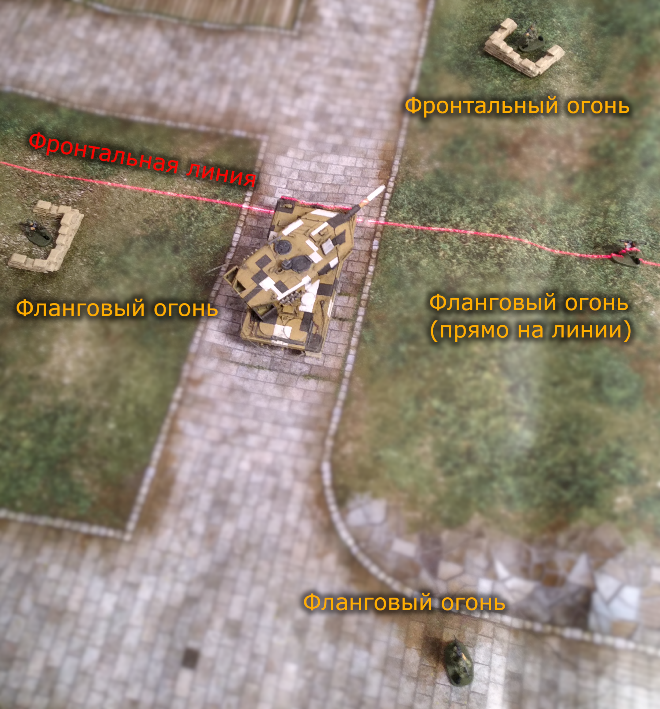
\includegraphics[width=\linewidth]{media/contract/image7.png}
\captionof{figure}{ориентация и фронтальная линия}
\end{minipage}

Фронтальная линия --- это линия, перпендикулярная вектору ориентации
боевой единицы и проходящая через точку, которая выбрана как точка
отсчёта для боевой единицы (например, середина переднего края корпуса
при использовании крупных фигурок). Таким образом, фронтальная линия
делит игровую плоскость на две части: одна часть, на которой стоит сама
боевая единица, считается находящейся \textbf{за} фронтальной линией, а
вторая часть --- \textbf{перед} фронтальной линией и перед боевой
единицей. По этой боевой единице враги, находящиеся перед фронтальной
линией, ведут фронтальный огонь (атака «в лоб»), а те, что находятся за
фронтальной линией ведут фланговый огонь (атака во фланг или с тыла).

\subsubsection{Линии видимости и огня}\label{los}

В игре используется понятие линии видимости при определении возможностей
наблюдать вражескую боевую единицу и открывать огонь по ней. Линия
видимости и линия огня --- это тождественные понятия. Линию видимости
следует проводить между заранее определёнными точками боевых единиц.

Линия видимости проводится в горизонтальной плоскости и может быть
прервана зонами локации, в том числе отдельными элементами.

\subsubsection{Маскировка}\label{camouflage}

Современный бой отличает большое количество средств разведки,
применяемых в реальном времени, таких как спутники, стратегические и
тактические БПЛА, благодаря которым командование может получать картинку
боя в реальном времени. Это соответствует тому, как командир видит все
боевые единицы на игровом поле боя, как свои, так и вражеские. Однако,
сами боевые единицы не всегда получают эту информацию в реальном
времени. И даже получив информацию о местонахождении противника,
требуется время на ориентацию по месту действия.

Боевая единица может быть замаскированной, и это означает, что
её не видят вражеские отряды и не могут открыть по ней прицельный
огонь\footnote{См. стр. \pageref{mod-blind}, \ref{mod-blind} \nameref{mod-blind}.}

Для того, чтобы боевая единица могла стать замаскированной,
необходимо выполнение одного из следующих условий:

\begin{enumerate}
\def\labelenumi{\arabic{enumi}.}
\item
  полное отсутствие линии видимости до всех вражеских боевых единиц;
\item
  прохождение всех линий видимости до вражеских боевых единиц через
  дымовую завесу.
\end{enumerate}

Маскировка сохраняется, в том числе и при передвижении боевой единицы.

Замаскированная боевая единица считается демаскированной (обнаруженной) в следующих случаях:

\begin{enumerate}
\def\labelenumi{\arabic{enumi}.}
\item
  замаскированная боевая единица вела огонь без использования
  звукоподавителей и пламегасителей;
\item
  замаскированная боевая единица успешно демаскирована
  вражеской боевой единицей в результате наблюдения\footnote{См. стр.~\pageref{observation}, \ref{observation}~\nameref{observation}.}.
\end{enumerate}

\subsubsection{Звук и звукоподавители}\label{sound}

Пехота вне городской локации может слышать звук вражеской техники, звуки
выстрелов и взрывов на дистанции до 150 см.

В городской локации звуки выстрелов и взрывов слышны на дистанции до 100
см, звук техники не учитывается.

Звукоподавители могут устанавливаться на некоторое пехотное оружие и
обеспечивают невозможность определения позиции замаскированного стрелка.

\subsubsection{Очки усталости}\label{fatigue}

У пехотных отрядов есть показатель усталости, который в начале игры
равен нулю. Пехота получает по одному очку усталости при передвижении
бегом и при преодолении препятствий. Очки усталости накапливаются, но не
могут быть больше уровня физической подготовки Ур(ВНС)\footnote{См. стр.~\pageref{endurance}, \ref{endurance}~\nameref{endurance}.} персонажа с самым маленьким Ур(ВНС) в
отряде. Это означает, что если в отряде есть персонаж, у которого
Ур(ВНС)~=~0, весь отряд не может передвигаться бегом и преодолевать препятствия.

Очки усталости уменьшаются на 1 в завершающую фазу хода\footnote{См. стр.~\pageref{end-phase}, \ref{end-phase}~\nameref{end-phase}.}, если отряд не передвигался или передвигался в
транспорте.

Если очки усталости отряда больше 0, при стрельбе персонажи отряда
должны использовать модификатор внезапного огня\footnote{См. стр.~\pageref{mod-sudden}, \ref{mod-sudden}~\nameref{mod-sudden}.}

\subsubsection{Очки стресса}\label{stress}

У отрядов есть показатель стресса, который в начале игры равен нулю.
Отряды получают очки стресса при обстреле. В пехотных отрядах очки
стресса распределяются равномерно по всем персонажам отряда. Они
накапливаются и в дальнейшем используются для определения возможности
исполнения действий.

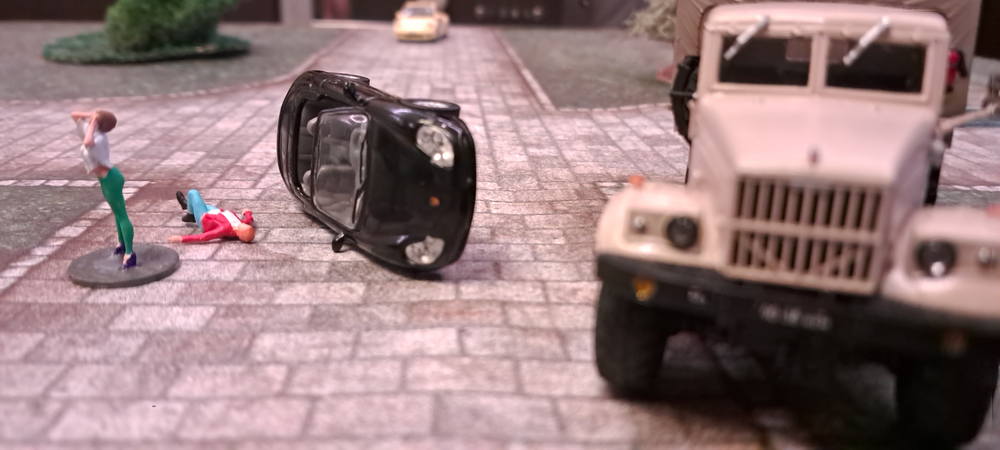
\includegraphics[width=\linewidth]{media/contract/image8.png}

Для пехотных отрядов каждое очко стресса (с округлением в большую
сторону) делает неэффективным одного солдата, но очки стресса могут
накапливаться свыше количества солдат в отряде. Это приводит к следующим
эффектам:

\begin{itemize}
\item
  неэффективные солдаты не могут участвовать в стрельбе и не
  могут выполнять наблюдение; неэффективными солдаты становятся
  по возрастанию $Макс(ЛГК/ВЛН)$ начиная от самого меньшего; если у
  нескольких солдат одинаковый $Макс(ЛГК/ВЛН)$, солдат выбирается
  случайно;
\item
  отряд, в котором неэффективны больше половины солдат, может двигаться
  только в сторону от врага, исключая замаскированные вражеские
  боевые единицы и не может выполнять штурм.
\end{itemize}

Стресс не влияет на возможность постановки дымовой завесы, на
возможность оказывать медицинскую помощь и на возможность использовать
средства связи.

Для отрядов на технике превышение количества очков стресса над значением
бронированности\footnote{См. стр. \pageref{table-armor}, \autoref{table-armor} \nameref{table-armor}.} приводит к тому,
что боевая единица может только двигаться на максимальной скорости в
сторону от врага, исключая \textbf{замаскированные} вражеские боевые
единицы. Если это действие выполнить невозможно, экипаж покидает
технику, но количество очков стресса у покинувшего технику отряда при
этом сохраняется.

\subsubsection{Кровотечение}\label{bleeding}

Раненый персонаж не может действовать, в том числе его навыки не
используются в игре. Например, его навык $Макс(ЛГК/ВЛН)$ не может быть
использован для восстановления очков стресса отряда. Единственное, что
может делать раненый персонаж --- это оказывать себе медицинскую помощь.

В завершающую фазу хода персонаж с кровотечением теряет 1 очко навыка
ВНС. Когда очки ВНС персонажа в завершающую фазу хода равны 0 и
кровотечение всё ещё действует, он умирает. Пока персонаж не умер,
кровотечение можно попытаться остановить с помощью навыка
МЕД\footnote{См. стр.~\pageref{medicine}, \ref{medicine}~\nameref{medicine}.}.

\section{Локация}\label{location}

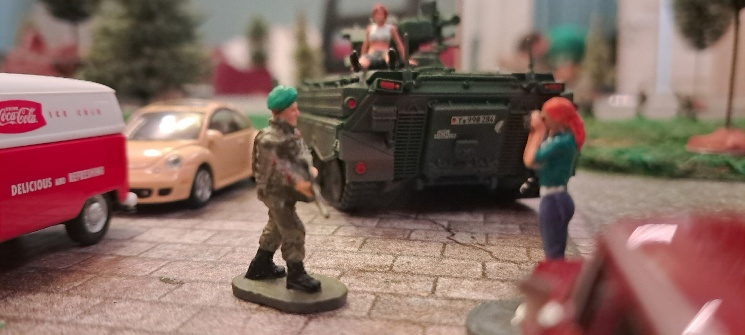
\includegraphics[width=\linewidth]{media/contract/image9.jpeg}

Игра происходит в определённой локации, представляющей из себя
плоскость, разделённую на зоны разных форм и размеров. Сценарий игры
должен подробно описывать локацию и все зоны, которые в ней
используются, включая их расположение и все их характеристики.

Автор использует стандартный размер игрового поля для игры с
миниатюрами: 180 см в длину и 120 см в ширину. Такое поле можно
разместить на столе в небольшой комнате.

Масштаб игры таков, что зона поражения артиллерии и даже миномётов может
покрыть всю игровую область, поэтому в большинстве сценариев артиллерия
может быть расположена за игровой областью. В некоторых сценариях игрок
как командир тоже может действовать за игровой областью. Это означает,
что он управляет боем дистанционно из другого места.

Даже танки были бы способны вести огонь через всю локацию, если бы она
представляла собой ровное поле. По этой причине, если, конечно, ваш
сценарий не предполагает масштабного танкового боя, наподобие битвы на
73 истинг, необходимо обеспечить высокое насыщение игрового поля
различными элементами локации и стараться не оставлять без особой
необходимости пустых пространств более 10 см. При недостатке элементов
локации можно использовать лесные зоны, задаваемые полигонами.

Следует избегать ситуаций, когда одна из боевых единиц, находящаяся в
локации, вынуждена вести прямой бой с боевой единицей, находящейся за
пределами локации. Это неудобно и может сильно испортить впечатление от
игры, потому что игроки могут неправильно представлять контекст вне
локации. Для этого очень важно располагать цели сценария ближе к
середине локации и обеспечить отсутствие линий видимости и хорошей
проходимости (по крайней мере для техники) непосредственно от края
локации по направлению к целям сценария. При создании локации следует
явно оговорить, что происходит, когда боевые единицы достигают границы
или выходят за неё.

Например, танк и ПТРК могут перестреливаться на дистанции более 200 см в
игровом масштабе. Если ПТРК занимает позицию на прямой дороге недалеко
от края локации, например в 50 см, и эта дорога продолжается по прямой
за границей локации, то фактически танку не будет смысла приближаться к
цели настолько, чтобы его можно было отобразить в локации. Следует
договориться, что, например, на границе локации дороги делают поворот, а
вокруг густые джунгли или плотная городская застройка, или локация
находится на плато, поэтому танку необходимо преодолеть склон, чтобы
иметь возможность вести огонь прямой наводкой. Таким образом, участники
договариваются, что прямой бой невозможен, если одна из боевых единиц не
находится в пределах локации.

\subsection{Зоны локации}\label{zones}

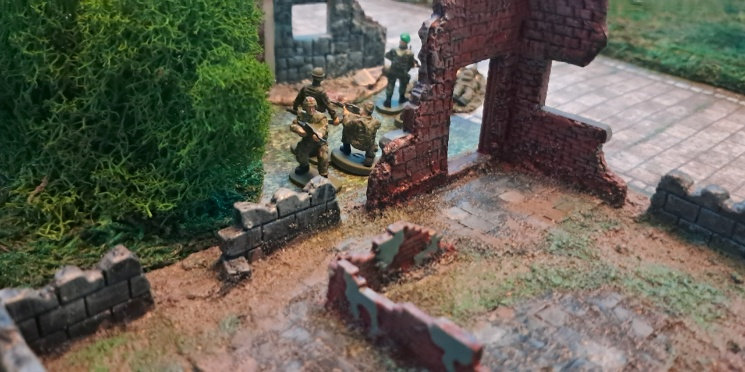
\includegraphics[width=\linewidth]{media/contract/image10.png}

\subsubsection{Стандартные зоны локации}\label{std-zones}

\begin{itemize}
\item
  Открытая местность. По умолчанию всё является открытой местностью.
\item
  Водные зоны. Не прерывают линию видимости. Непроходимы для техники и
  пехоты. Примеры: реки, озёра, болота.
\item
  Дороги. Позволяют технике быстрее передвигаться, никак не влияют на
  пехоту. Мост считается дорогой. Брод считается открытой местностью с
  препятствием. Ни то, ни другое не влияет на линию видимости.
\item
  Лес. Не разрушаем. Прохождение линии огня по зоне леса 3 см и менее
  приравнивается к среднему укрытию. Прохождение линии
  видимости по зоне леса непрерывно 3 см и более приводит к отсутствию
  видимости. Техника не может двигаться сквозь лес, но может быть
  замаскирована на кромке леса (прямо на границе лесной зоны).
  Техника может двигаться по границе лесной зоны, сохраняя
  маскировку.
\item
  Возвышение (холм). Считается открытой местностью, кроме случая, когда
  линия видимости пересекает границу одной зоны два раза (то есть боевые
  единицы находятся по разные стороны холма). В таком случае линии
  видимости нет. Граница холма или часть границы может быть совершенно
  непроходимой (скала, утёс).
\end{itemize}

\subsubsection{Дополнительные элементы}\label{elements}

Дополнительные элементы --- это небольшие зоны сложной геометрической формы с особыми свойствами,
которые могут быть описаны в сценарии. Должны быть описаны следующие свойства:

\begin{itemize}
\item
  разрушаемость: можно задать минимальную бронебойность (ББ) оружия для
  разрушения\footnote{См. стр. \pageref{infantry-weapons}, \ref{infantry-weapons} \nameref{infantry-weapons}.};
\item
  прерывает ли линию видимости;
\item
  отдельный элемент, не прерывающий линию видимости, как правило
  является укрытием, маскирует боевые единицы и может
  влиять на вероятность поражения. Укрытия\footnote{См. стр. \pageref{mod-cover}, \ref{mod-cover} \nameref{mod-cover}.} бывают нескольких видов:
  \textbf{маскирующие}, \textbf{средние} и \textbf{надёжные}, они
  отличаются степенью защиты.
\item
  проходимость отдельно для техники и пехоты (не проходимо,
  препятствие или легко проходимо); обычно,
  препятствия для техники легко проходимы для пехоты, а
  препятствия для пехоты могут быть как легко проходимыми для
  техники (например, колючая проволока), так и быть непроходимыми для
  неё (например, руины здания).
\end{itemize}

\paragraph{Примеры дополнительных элементов}\label{element-examples}

Окоп. Не разрушаем, является препятствием для техники, не прерывает
линию видимости, является надёжным укрытием для полностью
находящихся внутри контура. Техника тоже может получить надёжное
укрытие, если полностью помещается в окоп.

Глухой высокий бетонный или кирпичный забор: прерывает линию видимости,
не разрушаем, не проходим для техники, препятствие для пехоты.

Мешки с песком: не прерывают линию видимости, не разрушаемы, являются
препятствием для техники, легко проходимы для пехоты, являются
средним укрытием.

Толстый невысокий кирпичный забор или оконный проём здания: не
разрушаемы, не прерывают линию видимости, не проходимы для техники,
легко проходимы для пехоты, являются средним укрытием.

Здания определяются своим профилем в горизонтальной плоскости, состоящим
из сегментов разных элементов: глухие стены (прерывают линию видимости,
неразрушаемы, непроходимы, но могут быть препятствием для
пехоты если нет крыши), окна, двери, проломы в стенах (не прерывают
линию видимости, не разрушаемы, непроходимы для техники, легко проходимы
для пехоты, являются средним укрытием), амбразуры (то
же самое, что окна, но непроходимы и являются надёжным
укрытием).

\section{Симуляция боя}\label{combat}

В бою участвуют две стороны или более. На каждой стороне в бою могут
участвовать один или несколько игроков-командиров, у каждого из которых
в подчинении свои отряды.

Сценарий игры должен определять стороны, локацию, количество командиров
и состав подчинённых им отрядов, их начальное расположение, максимальное
количество ходов и прочие вводные. При создании сценария рекомендуется
ограничивать десятью количество боевых единиц у одного командира и
максимальное количество ходов.

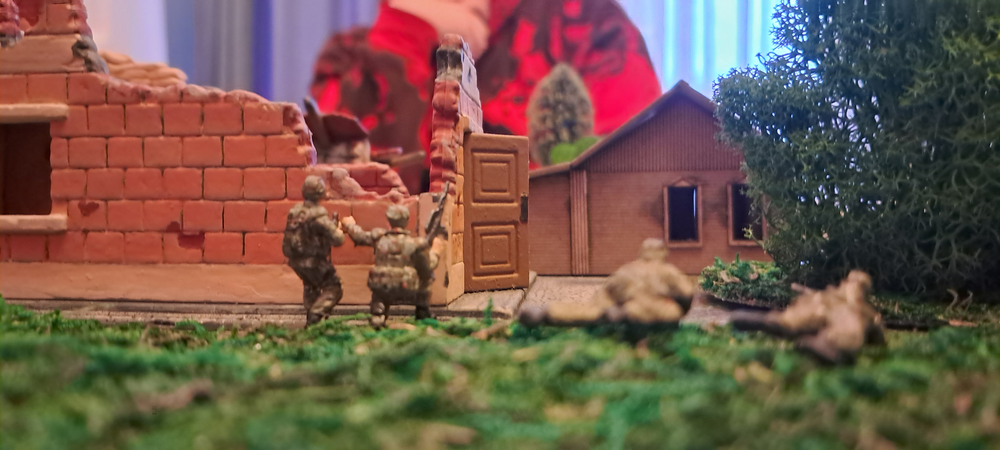
\includegraphics[width=\linewidth]{media/contract/image11.png}

Пошаговый тактический режим разделяется на ходы, каждый из
которых разделён на фазы:

\begin{enumerate}
\def\labelenumi{\arabic{enumi}.}
\item
  Фаза действий.
\item
  Завершающая фаза.
\end{enumerate}

После того, как все фазы завершены, ход завершается и начинается
следующий.

Бой начинается с устройства локации и расстановки отрядов. После этого
игроки могут заявлять действия в рамках упрощённого тактического
режима\footnote{См. стр. \pageref{game-modes}, \ref{game-modes} \nameref{game-modes}.} Учитывая заявки игроков, определяется момент, с которого
потребуется переключиться на пошаговый тактический режим и время,
которое пройдёт до этого момента с начала игры. Игроки могут параллельно
выполнить озвученные заявки длительностью не более рассчитанного
времени, после чего игра переходит в пошаговый тактический режим и
начинается новый \textbf{ход}.

Бой завершается по условию сценария или по соглашению игроков.

\subsection{Фаза действий}\label{action-phase}

В фазе действий игроки осуществляют действие по одной боевой единице в
порядке, определённом Макс(ЛГК/ВЛН) одного из персонажей отряда начиная
с наибольшего к наименьшему. Среди отрядов с одинаковым Макс(ЛГК/ВЛН)
порядок определяется случайно.

\subsubsection{Перехват движения}\label{intercept}

Когда в течение текущего хода вражеская боевая единица двигается в зоне
видимости дружественной боевой единицы, которая в этом ходу не выполняла
никаких действий, это движение может быть остановлено игроком в
произвольном месте. Один из персонажей этой дружественной единицы должен
провести наблюдение и, если оно будет успешно, другие персонажи смогут
осуществить стрельбу. После этого прерванное действие вражеской боевой
единицы может быть продолжено. При продолжении прерванного действия
следует учесть изменение очков стресса.

При стрельбе во время перехвата действия должен быть применён
модификатор внезапного огня\footnote{См. стр. \pageref{mod-sudden}, \ref{mod-sudden} \nameref{mod-sudden}.}

Перехват движения может выполняться боевой единицей только один раз за
ход. Перехват движения считается действием отряда, то есть отряд уже не
будет действовать в свою очередь в порядке инициативы.

\subsection{Завершающая фаза}\label{end-phase}

Происходит объединение отрядов, если отряды к этому моменту находятся в
одной точке и объединение заявлено игроком. При этом очки стресса
суммируются, а очки усталости берутся равными максимальному значению у
разделённых отрядов.

В завершающей фазе дымовые завесы проходят проверку на рассеивание. Для
каждой дымовой завесы сделать бросок D20, на 14+ дымовая завеса
рассеивается.

Каждый отряд восстанавливает некоторое количество очков стресса, в
соответствии с уровнем навыка лидерства Ур(Макс(ЛГК/ВЛН)).

\begin{center}
\begin{minipage}{0.7\columnwidth}
\begin{talltblr}[
  caption = {Восстановление очков стресса},
  label = {table-stress-recovery}
]{
  hlines,
  row{odd}={fg=navy},
  row{even}={fg=black},
  colspec={ Q[c,m,co=1] Q[c,m,co=1] },
}
\SetRow{font=\footnotesize}Восстановление очков стресса & Уровень навыка Ур(Макс(ЛГК/ВЛН)) \\
0,1 & 0 \\
0,2 & 1 \\
0,5 & 2 \\
0,8 & 3 \\
1,3 & 4 \\
1,9 & 5 \\
2,7 & 6 \\
\end{talltblr}
\end{minipage}
\end{center}

Персонажи с кровотечением теряют 1 очко навыка ВНС, а если количество
очков ВНС персонажа уже 0 к этому времени, такой персонаж умирает.

\section{Действия}\label{actions}

\subsection{Разделение отряда}\label{split-squad}

Разделение отряда может произойти перед его действием. При разделении
отряда очки стресса должны быть разделены между новыми отрядами
пропорционально количеству персонажей в отрядах, так, чтобы их сумма
осталась неизменной. Очки усталости отрядов равны очкам усталости
исходного отряда. После разделения отряды сразу же могут действовать
раздельно.

\subsection{Движение отряда}\label{movement}

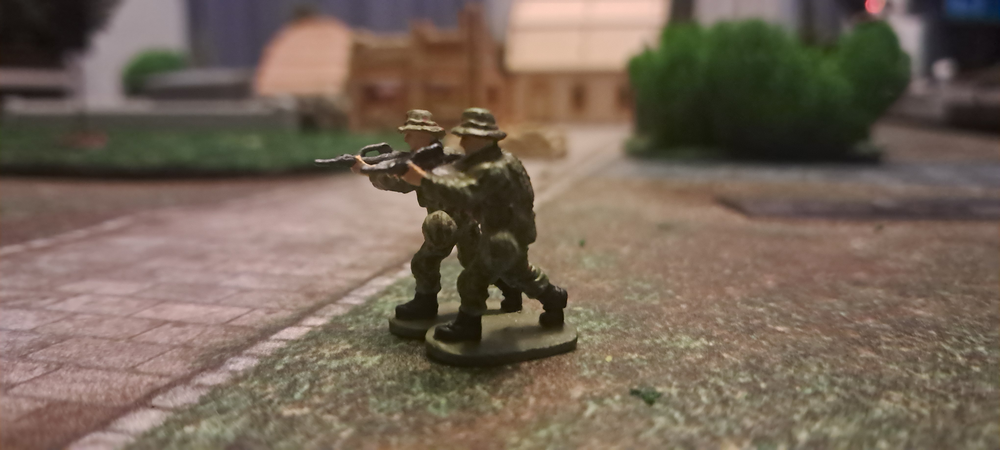
\includegraphics[width=\linewidth]{media/contract/image12.png}

Отряд двигается как единое целое.

Некоторые действия персонажей совместимы с движением отряда в том же
ходу, а некоторые возможны только при отсутствии движения в том же ходу.

Боевая единица с маркером стационарного положения не может двигаться.

Техника и пехота двигается на расстояние, зависящее от типа местности.
При прохождении маршрута через разную местность для расчёта расстояния
выбирается худший случай.

\setlength\rotheadsize{1.9cm}
\begin{minipage}{\columnwidth}
\begin{talltblr}[
  note{1}={\footnotesize См. стр. \pageref{table-movement}, \autoref{table-movement} \nameref{table-movement}.},
  caption = {Дальность движения за ход и значения для броска кубиков при преодолении препятствий},
  label = {table-vehicle-movement}
]{
  hlines,
  row{odd}={fg=navy},
  row{even}={fg=black},
  colspec={Q[c,m,co=3] Q[c,m,co=1] Q[c,m,co=1] Q[c,m,co=1]}
}
\SetRow{font=\footnotesize}& \rothead{Открытая\\местность} & \rothead{Дорога} & \rothead{Проверка на\\управление} \\
Пехота &
\SetCell[c=2]{c,m}{2--5~см\TblrNote{1}} & --- \\
Гусеничные БМ & 12 см & 16 см & 10+ \\
Колёсные БМ & 12 см & 16 см & 20+ \\
Автомобиль & 6 см & 20 см & 30+ \\
Вертолёт & \SetCell[c=2]{c,m}{50 см} & 15+ \\
Самолёт & \SetCell[c=2]{c,m}{150 см} & 13+ \\
\end{talltblr}
\end{minipage}

При выполнении действия следует положить рядом с боевой единицей маркер
движения, его можно будет убрать при следующей активации боевой единицы.

\subsubsection{Особенности движения наземной техники}\label{vehicle-movement}

Гусеничная техника в рамках одного действия двигается только по прямой,
а колёсная может изменять направление во время движения 1 раз.
После передвижения техника должна быть ориентирована по
направлению движения.

В начале любого действия техника может поворачиваться на любой угол.

Если у экипажа техники, выполняющей движение, количество очков стресса
больше показателя брони\footnote{См. стр.~\pageref{table-armor}, \autoref{table-armor}~\nameref{table-armor}.} она не
может приближаться к \textbf{демаскированным} вражеским отрядам, но
может отдаляться от них. Если это условие выполнить невозможно, то
экипаж покидает технику.

Техника может максимально ускориться и двигаться в два раза быстрее, чем
обычно, но только на идеальной дороге при движении по прямой. При любом
изменении направления относительно направления начала движения или при
движении не по дороге водитель должен пройти проверку на управление.

При движении через \textbf{препятствия} техника движется как по открытой
местности, но должна пройти проверку на управление.

\subsubsection{Особенности движения воздушной техники}\label{air-vehicle-movement}

Воздушная техника игнорирует ограничения наземной местности (лес,
здания, баррикады), но при этом пилот должен проходить проверки на
управление при выполнении каждого манёвра.

Манёвры для самолёта: взлёт, посадка, атака неуправляемым оружием.

Манёвры для вертолёта: взлёт, посадка, зависание, атака неуправляемым оружием. Проверку на зависание нужно проходить всегда,
за исключением случая, когда вертолёт передвигается на максимальную дистанцию.

При провале проверки на управление при взлёте или посадке происходит крушение.

При провале проверки на атаку неуправляемым оружием стрельба не происходит.

При провале проверки на зависание на месте при управлении вертолётом он должен сместиться на максимальную дистанцию
в случайном направлении от начального положения.

Самолёт может двигаться только по прямой в рамках одного действия, при этом он всегда перемещается на полное расстояние,
если только он не осуществляет посадку.

В начале любого действия воздушная техника может изменить направление на любой угол.

\paragraph{Таран}\label{ramming}

Водитель, желающий осуществить таран, должен пройти проверку на управление.

При успехе, смоделировать обоюдные удары по технике по правилам выстрела,
используя в качестве значения Бронебойности (ББ) значение Бронированности, увеличенное на 1.
Обе единицы техники должны пройти проверку на управление в следующий ход.

Рядом с машиной необходимо положить маркер обездвиженности.

\paragraph{Проверка на управление}\label{control-check}

Бросить кубик D20, к результату броска прибавить очки тренированности навыка
МЕХ\footnote{См. стр. \pageref{mechanics}, \ref{mechanics} \nameref{mechanics}.}, итоговый результат сравнить со значением из
таблицы (\autoref{table-vehicle-movement}). Если выпало меньше --- проверка не пройдена.

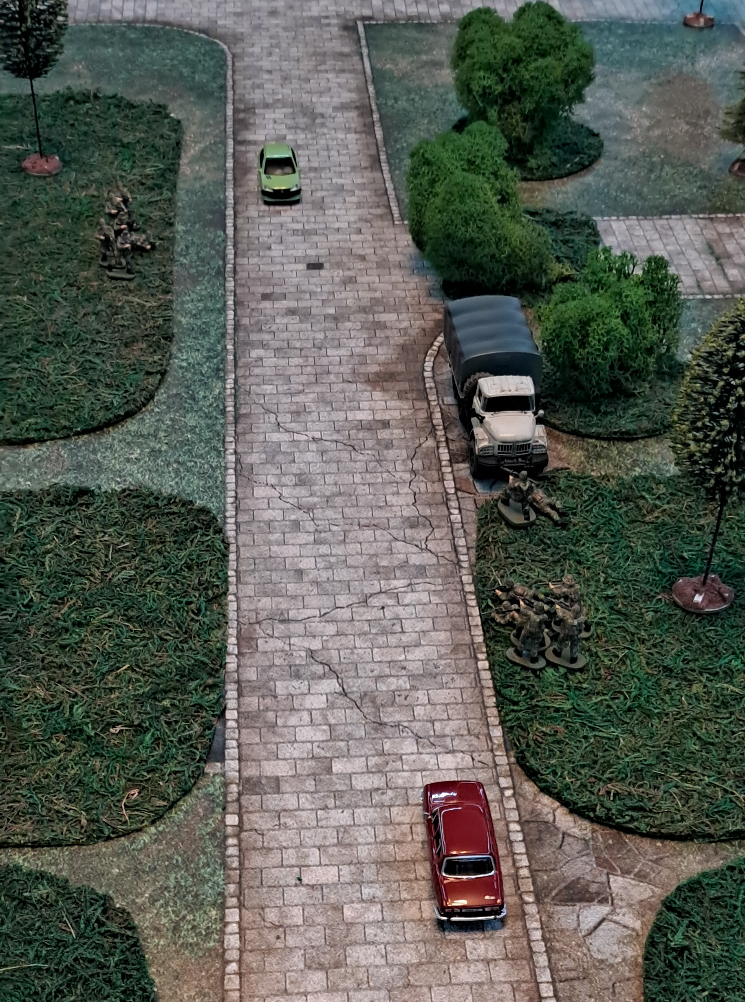
\includegraphics[width=\linewidth]{media/contract/image13.png}

\paragraph{Пример}\label{example-endurance-1}

БТР-82А пытается прорваться через баррикаду. Прорыв успешен при
выбрасывании 20 и выше. Мехвод БТР имеет 7 очков тренированности МЕХ.
Это уменьшает требуемый порог: $20 - 7 = 13$. При выбрасывании меньше 13
БТР останавливается перед баррикадой. В следующий ход десант,
находящийся в БТР, может высадиться из него, при этом передвинуться на
соответствующее расстояние от БТР. В этот же момент другой отряд пехоты
может осуществить посадку в этот же БТР, если расстояние до него не
более максимальной дальности движения.

\subsubsection{Особенности движения пехоты}\label{infantry-movement}

Если у пехотного отряда, выполняющего движение, количество очков
стресса больше половины численности отряда, он не может
приближаться к \textbf{демаскированным} вражеским отрядам, но может
отдаляться от них. Если это условие выполнить невозможно, то отряд не
может двигаться.

Для передвижения отряда с ранеными персонажами с кровотечением на
каждого раненого персонажа в отряде должен приходиться здоровый
персонаж, так как раненым требуется помощь.

\paragraph{Бег}\label{running}

При беге отряд пехоты может двигаться в два раза быстрее, чем обычно,
после чего получит по 1 очко усталости.

Бег возможен только если количество очков усталости в отряде меньше, чем
минимальное значение Ур(ВНС) у персонажей этого отряда.

\paragraph{Преодоление препятствий}\label{obstacles}

Преодоление препятствия для отряда пехоты возможно только если
количество очков усталости в отряде меньше, чем минимальное значение
Ур(ВНС) у персонажей этого отряда. При преодолении препятствия отряд
получает 1 очко усталости.

Следует помнить, что то, что является препятствием для техники
может быть легко проходимо для пехоты (например, противотанковые ежи),
такие элементы не влияют на движение пехоты.

\paragraph{Посадка и высадка}\label{boarding-disembark}

При движении пехотные отряды могут осуществлять посадку в технику и
высадку из неё. Для посадки точка назначения для движения должна быть на
технике, при высадке точка назначения может быть где угодно в пределах
дальности движения. Посадка и высадка несовместима с движением техники в
том же ходу. Это же правило применяется для экипажа техники.

\subsection{Действия персонажей}\label{person-actions}

Персонажи в отряде могут действовать раздельно: наблюдать, вести огонь по разным целям, оказывать помощь раненым.
Некоторые действия персонажа можно выполнить во время движения отряда, а некоторые требуют остановки:
короткой (отряд не должен перемещаться в текущем ходу) или длительной (отряд не должен перемещаться в прошлом, текущем и следующем ходах)
\footnote{См. стр. \pageref{stationary-position}, \ref{stationary-position} \nameref{stationary-position}.}.

\subsubsection{Наблюдение}\label{observation}

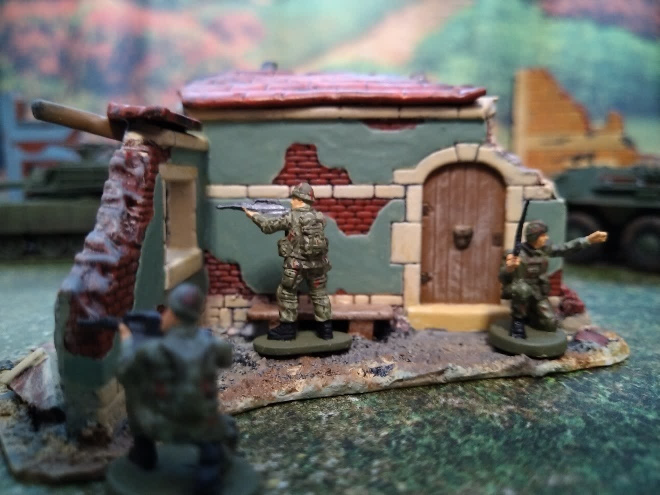
\includegraphics[width=\linewidth]{media/contract/image14.png}

Для того, чтобы обнаружить замаскированную боевую единицу,
необходимо пройти проверку, учитывая условия видимости.

В рамках одного хода и одного отряда наблюдение за выбранной целью может
вести только один персонаж. Другие персонажи отряда могут вести
наблюдение за другими боевыми единицами. Наблюдение может быть выполнено
до движения или после движения.

Базовое значение видимости и максимальная дальность видимости выбираются
по таблице исходя из текущих условий в сценарии (см. \autoref{table-visibility}). Если
одновременно действует несколько условий, выбираются минимальные
значения отдельно по дальности, отдельно по видимости.

Ночью боевые единицы, находящиеся в освещённых местах, видны как днём.

Если для наблюдения используется снаряжение, то следует применить
модификатор видимости от снаряжения (см. \autoref{table-visibility-equipment}) по всем условиям.
Максимальная дальность для каждого условия должна быть использована от
снаряжения. Из нескольких условий всё равно должны быть выбраны
минимальные значения отдельно по дальности, отдельно по видимости.

Технику заметить гораздо проще, чем пехоту, поэтому при наблюдении
техники максимальная дальность удваивается, удваивается дальность
обнаружения в таблице пороговых значений (см. \autoref{table-recon-thresholds}), а на
расстоянии до 3 см техника обнаруживается автоматически.

Если цель находится в укрытии любого типа, от выбранного
модифицированного значения видимости необходимо отнять 5.

К модифицированному значению следует прибавить навык маскировки
наблюдателя $Ур(МСК)$.

Если для наблюдения используется дрон, к модифицированному значению
следует прибавить уровень навыка управления дронами наблюдателя $Ур(ДРН)$,
в противном случае прибавить навык маскировки наблюдателя $Ур(МСК)$ второй
раз.

При наблюдении за отрядом пехоты нужно отнять удвоенный навык маскировки
цели $Ур(МСК)$\footnote{См. стр. \pageref{camouflage-skill}, \ref{camouflage-skill} \nameref{camouflage-skill}.}
(выбирается минимальный МСК из персонажей отряда).

После этого к модифицированному значению прибавить результат броска D20
и получившееся значение сравнить с пороговыми значениями (см. \autoref{table-recon-thresholds}).

\begin{minipage}{\columnwidth}
\begin{talltblr}[
  caption = {Базовое значение видимости и дальность видимости},
  label = {table-visibility}
]{
  hlines,
  row{odd}={fg=navy},
  row{even}={fg=black},
  colspec={ Q[c,m, co=0.3324] Q[c,m, co=0.3509] Q[c,m, co=0.3166] },
}
\SetRow{font=\footnotesize}Условия & Базовое значение видимости & Макс. дальность видимости, см \\
Ясный день & 12 & 160 \\
Сумерки & 7 & 80 \\
Ночь & 2 & 16 \\
Сильные осадки & 8 & 40 \\
Туман & 7 & 6 \\
\end{talltblr}
\end{minipage}

\setlength\rotheadsize{2.3cm}
\begin{minipage}{\columnwidth}
\begin{talltblr}[
  caption = {Модификатор видимости от снаряжения},
  label = {table-visibility-equipment}
]{
  hlines,
  row{odd}={fg=navy},
  row{even}={fg=black},
  colspec={ Q[c,m,co=3]Q[c,m,co=2]Q[c,m,co=1]Q[c,m,co=1] },
}
Предмет & Условие & \rothead{Модификатор\\видимости} & \rothead{Макс.\\дальность\\видимости, см} \\
\SetCell[r=2]{l} Бинокль & День & +5 & 320 \\
& Сумерки & +2 & 160 \\
\SetCell[r=2]{l} Прибор ночного видения & Сумерки & +3 & 80 \\
& Ночь & +9 & 80 \\
\SetCell[r=5]{l} Тепловизионный прицел & День & +3 & 120 \\
& Сумерки & +4 & 140 \\
& Ночь & +12 & 160 \\
& Осадки & +4 & 20 \\
& Туман & +4 & 6 \\
\end{talltblr}
\end{minipage}

Если противник находится под крышей, то его невозможно обнаружить БПЛА с радиоуправлением, только БПЛА с оптоволоконным каналом связи.

При поиске ловушек и мин не применяется модификатор укрытия. Ловушки и мины невозможно обнаружить с воздуха.

\begin{center}
\begin{minipage}{0.7\columnwidth}
\begin{talltblr}[
  caption = {Пороговые значения для броска кубика при проведении разведки},
  label = {table-recon-thresholds}
]{
  hlines,
  row{odd}={fg=navy},
  row{even}={fg=black},
  colspec={ Q[c,m,co=1] Q[c,m,co=1] },
}
\SetRow{font=\footnotesize}Дистанция обнаружения, см & Модифицированный результат \\
3 & 10+ \\
10 & 17+ \\
20 & 22+ \\
40 & 27+ \\
80 & 32+ \\
160 & 37+ \\
320 & 42+ \\
Поиск мин (0--1) & 22+ \\
\end{talltblr}
\end{minipage}
\end{center}

\paragraph{Пример}\label{example-endurance-2}

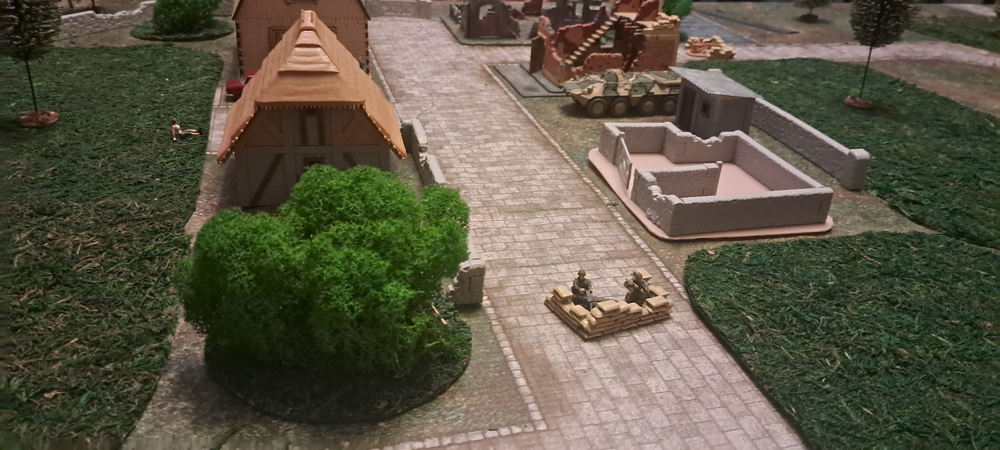
\includegraphics[width=\linewidth]{media/contract/image15.png}

Отделение панцергренадёров днём ведёт разведку населённого пункта, где в
здании укрылись солдаты противника.

Наблюдатель использует бинокль. Параметры при этом: видимость
$12+5=17$, максимальная дальность видимости 320. У наблюдателя
$Ур(МСК)=3$, поэтому итоговый модификатор наблюдателя $17+2×3=23$.
Это значение, которое нужно прибавить к результату броска.

У цели $Ур(МСК)=1$, кроме того, линия видимости пересекает стену с
окном. В игре по соглашению применяется метод неравномерного
пространства\footnote{См. стр.~\pageref{miniatures}, \ref{miniatures}~\nameref{miniatures}.}, поэтому стена считается средним
укрытием\footnote{См. стр.~\pageref{element-examples}, \ref{element-examples}~\nameref{element-examples}.}, следовательно, применяется
модификатор -5. Итого модификатор цели $(-5)-1×2=-7$. Это значение,
которое нужно будет вычесть из результата броска.

Наблюдатель делает бросок D20. Допустим, выпадает 10. Итоговый результат
$10+23-7=26$. Дистанция 20 см, на этой дистанции результат должен
быть 22+. Можно объявить, что цель демаскирована.

В худшем случае, при выбрасывании 1, результат будет $1+23-7=17$.
То есть в данных условиях этот наблюдатель может автоматически
обнаружить такую цель на дистанции до 10 см. В лучшем случае, при
выбрасывании 20, результат будет $20+23-7=36$. Это означает, что в
данных условиях этот наблюдатель не сможет обнаружить такую цель на
дистанции свыше 80 см.

Если бы при этом шёл дождь, то бинокль невозможно было бы использовать
(для него не заданы модификаторы для дождя). Значение видимости было бы
$8+2×3-5-2×1=7$. В лучшем случае наблюдатель заметит
противника на дистанции до 40 см, а в худшем --- вообще не заметит.

\subsubsection{Стрельба}\label{shooting}

Каждый персонаж может вести огонь по отдельной цели. Примеры:
гранатомётчик отделения ведёт огонь по бронетранспортёру, а остальные
солдаты по вражескому пехотному отряду; один из пулемётов на
бронетранспортёре стреляет по одному отряду, а второй~-- по второму.

Если у отряда есть очки стресса, то часть персонажей не может вести
огонь\footnote{См. стр.~\pageref{stress}, \ref{stress}~\nameref{stress}.}

Оружие, стреляющее прямой наводкой, можно применять только при наличии
линии видимости от атакующего отряда к атакуемому\footnote{См. стр.~\pageref{los}, \ref{los}~\nameref{los}.}

Расстояние от атакующей боевой единицы до цели не должно превышать
максимальной дальности стрельбы оружия и максимальной дальности
видимости персонажа с учётом времени суток, погодных условий и
используемой экипировки и прицельных приспособлений. Например, несмотря
на то, что снайперская винтовка с оптическим прицелом позволила бы
стрелять на расстояние до 150~см и обнаруживать противника на расстоянии
до 320~см, ночью по неосвещённой цели из неё можно выстрелить только на
20 см. Однако, освещённую цель и ночью можно обнаружить на дистанции до
320 см, а цель, ведшую стрельбу с текущей позиции без пламегасителей
также видно на максимальном расстоянии, при этом она
демаскируется автоматически и проводить наблюдение не требуется.

Результат стрельбы определяется броском кубика D20 отдельно для каждого
используемого оружия, но по-разному при стрельбе по отрядам пехоты и по
технике.

\paragraph{Особенности стрельбы по пехоте}\label{infantry-shooting}

Сначала необходимо определить интенсивность огня (\textbf{ИО})
используемого оружия\footnote{См. стр. \pageref{table-infantry-weapons}, \autoref{table-infantry-weapons} \nameref{table-infantry-weapons}
и стр. \pageref{table-vehicle-weapons}, \autoref{table-vehicle-weapons} \nameref{table-vehicle-weapons}.}

Затем, используя параметр \textbf{ИО} и, если уместно, применив к
результату броска D20 модификатор флангового огня, определить количество
очков стресса, которые получит цель (см. \autoref{table-stress-from-fire}).

\begin{minipage}{\columnwidth}
\begin{talltblr}[
  caption = {Количество очков стресса при стрельбе},
  label = {table-stress-from-fire}
]{
  hlines,
  row{odd}={fg=navy},
  row{even}={fg=black},
  colspec={ Q[c,m,co=1]Q[c,m,co=1]Q[c,m,co=1] },
}
\SetRow{font=\footnotesize}Интенсивность Огня (ИО) оружия & Модифицированный результат броска & Количество очков стресса \\
1 & 15+ & 1 \\
2 & 11+ & 1 \\
2 & 20+ & 2 \\
3 & 8+ & 1 \\
3 & 17+ & 2 \\
3 & 20+ & 3 \\
4 & 6+ & 1 \\
4 & 16+ & 2 \\
4 & 19+ & 3 \\
4 & 20+ & 4 \\
\end{talltblr}
\end{minipage}

Затем также определяется количество поражённых солдат, но к результату
броска D20 применяются все модификаторы\footnote{См. стр.~\pageref{shooting-modifiers}, \ref{shooting-modifiers}~\nameref{shooting-modifiers}.}

\begin{minipage}{\columnwidth}
\begin{talltblr}[
  caption = {Количество раненых при стрельбе},
  label = {table-wounds-from-fire}
]{
  hlines,
  row{odd}={fg=navy},
  row{even}={fg=black},
  colspec={ Q[c,m,co=1]Q[c,m,co=1]Q[c,m,co=1] },
}
\SetRow{font=\footnotesize}Интенсивность Огня (ИО) оружия & Модифицированный результат броска & Количество раненых \\
1 & 16+ & 1 \\
2 & 13+ & 1 \\
2 & 21+ & 2 \\
3 & 11+ & 1 \\
3 & 20+ & 2 \\
4 & 9+ & 1 \\
4 & 19+ & 2 \\
4 & 22+ & 3 \\
\end{talltblr}
\end{minipage}

Распределение ран по персонажам отряда происходит среди персонажей, у
которых ещё нет кровотечения, в порядке возрастания очков
тренированности навыка МНВ с учётом наличия бронежилетов. Среди
персонажей с одинаковыми значениями выбор происходит случайно. Раненый
персонаж получает кровотечение, это нужно запомнить или записать.

\subparagraph{Пример}\label{example-endurance-3}

Отделение панцергренадёров ведёт огонь по отделению мотострелков. В
отделении панцергренадёров 6 солдат, один из которых вооружён ручным
пулемётом (\textbf{ИО} = 2), а остальные -- штурмовыми винтовками
(\textbf{ИО~}=~1).

Панцергренадёры имеют 5 очков тренированности ЛС, следовательно Ур(ЛС) =
2, а пулемётчик 7 очков тренированности ПЛМ, следовательно Ур(ПЛМ) = 3.
Среди мотострелков минимальное значение очков тренированности МНВ 4,
следовательно Ур(МНВ) = 2. Модификатор навыка для автоматчиков
$2×(2-2)=0$. Модификатор навыка для пулемётчика $2×(3-2)=2$.

Расстояние до цели 25 см. Это максимальная дальность для штурмовых
винтовок и эффективная дальность для пулемёта, поэтому автоматчики
получают модификатор расстояния -4.

Все панцергренадёры заняли удобную позицию для стрельбы и отряд имеет
модификатор стационарного положения. Но для автоматов он равен нулю, а
вот у пулемёта есть сошки, поэтому он получает +1.

В течение хода (30 секунд) отряд мотострелков не обстреливается
с других сторон, поэтому модификатор флангового огня не применяется.

Мотострелки находятся в здании с окнами, поэтому модификатор укрытия -2.

Отряд мотострелков был замечен панцергренадёрами ранее, поэтому
модификатор огня вслепую не применяется.

Панцергренадёры не уставшие, не запыхавшиеся, не были застигнуты
врасплох, поэтому модификатор внезапного огня не применяется.

Командир панцергренадёров бросает 6 кубиков D20, по одному за каждого
солдата.

Бросок 20+ за пулемётчика принесёт 2 очка стресса мотострелкам, а 11+
одно очко стресса. Бросок 15+ за каждого автоматчика принесёт ещё по
одному очку стресса мотострелкам.

Итоговый модификатор для определения количества ран для пулемётчика
будет +1, для автоматчиков -5. Следовательно, для пулемётчика бросок 20+
принесёт 2 раны отряду мотострелков, 12+ одну рану. Для автоматчика
такой огонь никогда не принесёт ран: даже если выпадет 20, с учётом
модификатора будет 15, а для нанесения раны нужно 16+. Однако, огонь
имеет смысл, потому что автоматчиков много и каждый из них имеет шанс в
30\% подавить мотострелков, чтобы затем, например, приблизиться ближе и
взять здание штурмом или забросать гранатами.

При нанесении ран выбираются мотострелки с минимальным значением очков
тренированности МНВ и у них начинается кровотечение.

\paragraph{Особенности стрельбы по технике}\label{vehicle-shooting}

Сначала необходимо определить показатель бронебойности оружия
(\textbf{ББ}) (\autoref{table-infantry-weapons}) и показатель бронированности цели
(\textbf{Бр}) (\autoref{table-armor}). По таблице определяются два пороговых значения: для уничтожения и
для увеличения очков стресса. Отсутствие значения в соответствующей
ячейке означает, что данный тип оружия не может уничтожить данную цель
или не может оказать воздействия на её экипаж --- такая стрельба не
приносит никакого результата.

К результату броска D20 необходимо применить модификаторы при
стрельбе\footnote{См. стр. \pageref{shooting-modifiers}, \ref{shooting-modifiers} \nameref{shooting-modifiers}.} и сравнить результат с пороговым
значением.

Если результат равен или превышает порог уничтожения, техника считается
уничтоженной и немедленно выходит из строя.

Если результат ниже порога уничтожения, но равен или превышает порог
стресса, экипаж техники получает очки стресса, равные разнице между ББ и
Бр.

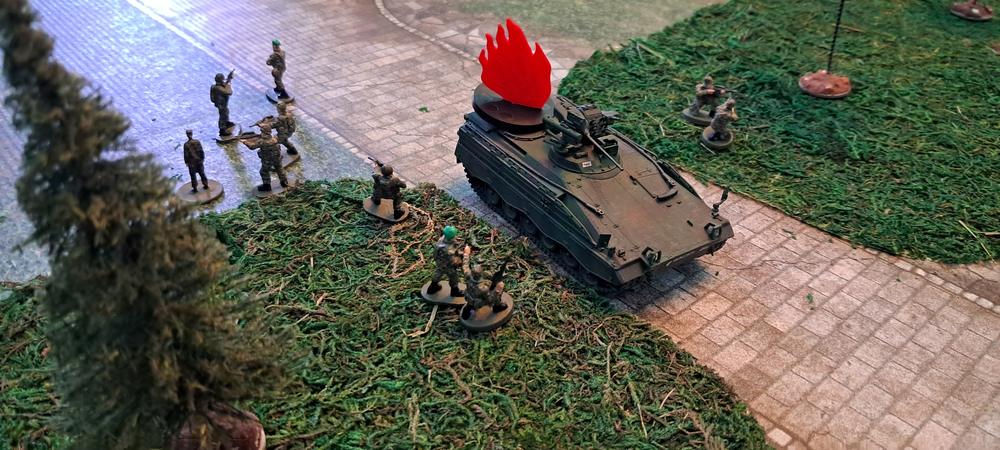
\includegraphics[width=\linewidth]{media/contract/image16.png}

\subparagraph{Поражение экипажа и десанта}\label{crew-injury}

В случае уничтожения единицы техники, экипаж и десант немедленно
выгружается. За каждого персонажа бросается кубик, у персонажа
начинается кровотечение на 14+, в противном случае добавляется +1 к
очкам стресса отряда.

\subparagraph{Пример}\label{example-endurance-4}

Танк M1A2 ведёт огонь по БМП M2A2. Бронированность БМП Бр~=~4,
бронебойность танковой пушки ББ~=~11. Базовые пороговые значения: на 7+
стресс, на 9+ уничтожение.

Наводчик пушки имеет 8 очков тренированности ТВ, следовательно
Ур(ТВ)~=~3, это и будет модификатором навыка.

Расстояние 100 см, для пушки это эффективная дальность.

Танк стреляет после движения, так что модификатор стационарного
положения не применяется.

Попадание потенциально придёт с фронта БМП, поэтому модификатор
флангового огня не применяется.

БМП находится в окопе, применяется модификатор укрытия -4.

Наводчик танка наблюдает БМП, поэтому модификаторы огня вслепую и
внезапного огня не применяются.

Итого, БМП будет уничтожена при выбрасывании 10+. Если же результат
окажется меньше, но 8+, БМП получит 7 очков стресса. Это означает, что
при следующей активации БМП её экипаж либо покинет машину, либо
попытается отступить с позиции на машине, либо будет сидеть следующие 30
секунд в машине, не в силах пошевелиться, но эффективно отбиваться уже
не сможет.

\paragraph{Стационарное положение}\label{stationary-position}

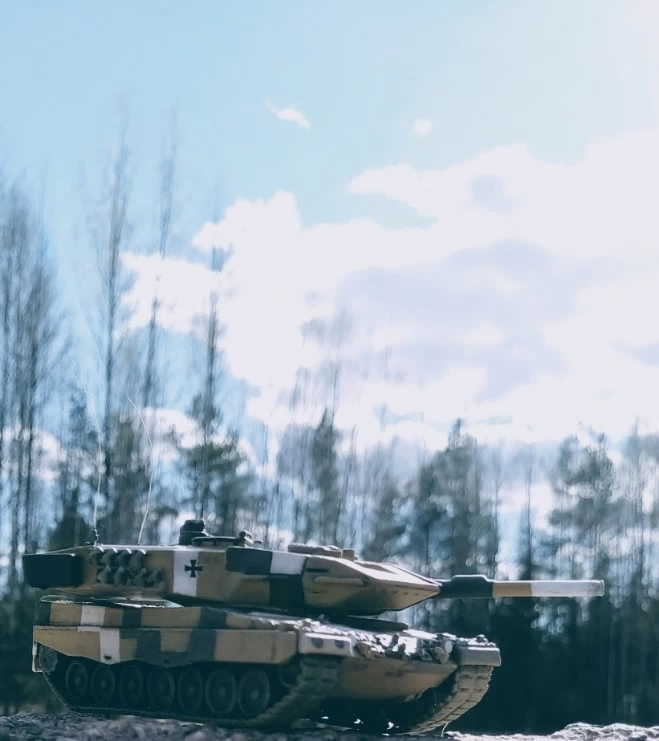
\includegraphics[width=\linewidth]{media/contract/image17.png}

Стационарное положение означает подготовку позиции и оружия к стрельбе и
позволяет вести огонь с большей эффективностью, но требует некоторого
времени для этой подготовки.

Боевая единица может считаться находящейся в стационарном положении если
она \textbf{не двигалась в предыдущем ходу}. При осуществлении
стрельбы из стационарного положения у боевой единицы не должно быть
маркера движения, а также следует положить рядом с боевой единицей
маркер стационарного положения, его можно будет убрать при следующей
активации этой боевой единицы. Таким образом, боевая единица,
находящаяся в стационарном положении, \textbf{не сможет двигаться в
следующем ходу}.

\paragraph{Модификаторы при стрельбе}\label{shooting-modifiers}

Модификаторы прибавляются к результату броска кубика. Они нужны для
того, чтобы учесть больше условий в вероятности возникновения события.
Одновременно могут применяться несколько модификаторов.

\subparagraph{Модификатор навыка}\label{mod-skill}

Модификатор навыка применяется по-разному для обстрела техники и пехоты.

При обстреле пехоты вычисляется удвоенная разница между навыком владения
используемым оружием атакующего Ур(X) и навыком маневрирования Ур(МНВ)
цели, эта разница прибавляется к результату броска. При определении
Ур(МНВ) цели выбирается минимальное значение Ур(МНВ) среди персонажей
отряда.

При обстреле техники используется только навык владения используемым
оружием атакующего Ур(X), он прибавляется к результату броска.

\subparagraph{Модификатор расстояния}\label{mod-range}

У некоторого оружия помимо максимальной дальности есть ещё идеальная и
эффективная дальность. Для такого оружия вероятность попадания
увеличивается с уменьшением расстояния до цели.

При расстоянии до цели в пределах идеальной дальности при броске кубика
нужно добавить 6 к результату броска, тем самым увеличив вероятность
попадания.

При расстоянии до цели свыше эффективной дальности нужно отнять 4 от
результата броска, тем самым уменьшив вероятность попадания.

Если у оружия обозначена только максимальная дальность, то это означает,
что модификатор расстояния можно не применять. Это, например,
снайперские винтовки и управляемые ракеты.

\subparagraph{Модификатор стационарного положения}\label{mod-stationary}

При стрельбе из стационарного положения на эффективной дальности оружия
вероятность попадания увеличивается на значение, определяемое
конфигурацией самого оружия. Модификаторы стационарного положения разных
частей оружия суммируются.

\subparagraph{Модификатор флангового огня}\label{mod-flank}

При обстреле техники c бронированностью Бр~\textgreater~2, если
атакующий отряд хотя бы частично находится за фронтальной линией
атакуемого\footnote{См. стр.~\pageref{position}, \ref{position}~\nameref{position}.}, то вероятность поражения
увеличивается. Необходимо прибавить 4 к результату броска.

Отряды пехоты не ориентированы, и фронтальная линия для них не
существует. Тем не менее, можно получить дополнительное преимущество,
обстреливая отряд пехоты с разных сторон. Если угол между линией огня и
любой другой линией огня, по которой обстреливался этот же отряд в этот
же ход, превышает 90°, то вероятность поражения увеличивается.
Необходимо прибавить 2 к результату броска.

\subparagraph{Модификатор огня вслепую}\label{mod-blind}

При стрельбе по необнаруженной\footnote{См. стр.~\pageref{observation}, \ref{observation}~\nameref{observation}.} \textbf{замаскированной} боевой единице вероятность
попадания существенно уменьшается. От результата броска нужно отнять 6.
Этот модификатор суммируется с модификатором укрытия.

\subparagraph{Модификатор внезапного огня}\label{mod-sudden}

При ведении внезапного огня при перехвате действия\footnote{См. стр.~\pageref{intercept}, \ref{intercept}~\nameref{intercept}.},
а также при наличии у отряда очков усталости, вероятность попадания
уменьшается. От результата броска нужно отнять 2.

\subparagraph{Модификатор укрытия}\label{mod-cover}

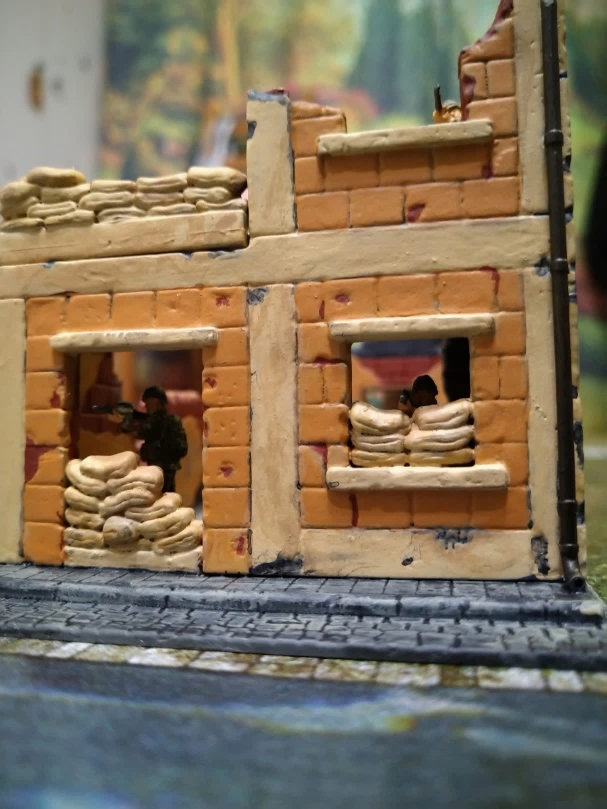
\includegraphics[width=\linewidth]{media/contract/image18.png}

Если линия огня пересекает укрытие (отдельный элемент или зону
леса шириной меньше 3 см), но не прерывается им, а атакующий находится
дальше 3 см от этого укрытия, то вероятность попадания
уменьшается.

От результата броска нужно отнять значение модификатора в соответствии с
типом укрытия (см. \autoref{table-cover-modifiers}).

\begin{center}
\begin{minipage}{0.7\columnwidth}
\begin{talltblr}[
  caption = {Значения модификаторов для типов укрытий},
  label = {table-cover-modifiers}
]{
  hlines,
  row{odd}={fg=navy},
  row{even}={fg=black},
  colspec={ Q[c,m,co=1] Q[c,m,co=1] }
}
Тип укрытия & Значение модификатора \\
Среднее & -2 \\
Надёжное & -4 \\
\end{talltblr}
\end{minipage}
\end{center}

\subparagraph{Модификатор бронежилета}\label{mod-bodyarmor}

Применяется только для пехотных отрядов.

Вычисляется средняя защита персонажей отряда: определяется сумма защиты
бронежилетов\footnote{См. стр.~\pageref{body-armor}, \ref{body-armor}~\nameref{body-armor}.}, используемых каждым персонажем отряда, и делится
на количество не раненых членов отряда. Округление в меньшую сторону.

Модификатор определяется как положительная разница между средней защитой
и параметра бронебойности ББ оружия. Этот модификатор вычитается из
результата броска.

Пример: из пулемёта обстреливается снайперская двойка. Снайпер имеет MSV
с плитами, а его напарник, наблюдатель --- полный MSV. Средняя защита отряда $(4+6)÷2=5$. ББ пулемёта M240 2, поэтому модификатор
$5-2=3$. Результат броска следует уменьшить на 3.

\subsubsection{Постановка дымовой завесы}\label{smoke}

Если у боевой единицы есть соответствующее вооружение (дымовые шашки у
персонажей или система запуска дымовых гранат на технике), то она может
поставить одну дымовую завесу с центром в пределах 4 см от точки своего
положения.

Диаметр дымовой завесы 5 см.

Дымовые завесы проходят проверку на рассеивание в завершающую фазу.

\subsubsection{Оказание медицинской помощи}\label{first-aid}

Остановка кровотечения у персонажа возможна, если рядом с ним есть
санитар или медик, то есть персонаж со значением навыка полевой медицины
больше 0. Медику необходимо пройти проверку навыка МЕД, бросив кубик D20
и к результату прибавив своё значение навыка полевой медицины Ур(МЕД).
Сложность оказания первой помощи с использованием Индивидуального Перевязочного Пакета 10+, без использования 20+.
Индивидуальный Перевязочный Пакет пропадает после использования.
При успешном броске у раненого солдата останавливается кровотечение, и
он может вернуться в игру с текущим значением очков навыка ВНС.

Один солдат с навыком полевой медицины может оказать помощь только
одному раненому за ход. Раненый с навыком медицины может попытаться
оказать помощь самому себе. Это действие не совместимо ни с каким
другим.

\subsection{Штурм и пленение}\label{assault}

Штурм применяется только для схватки между двумя пехотными отрядами, а
также для пленения солдат отряда с большим количеством очков стресса.

Штурм может быть объявлен только если отряд противника
обнаружен\footnote{См. стр.~\pageref{observation}, \ref{observation}~\nameref{observation}.} и расстояние до него равно 3 см и менее, при этом
отряды сближаются вплотную.

Штурм --- это одновременные удары отрядов, то есть потери применяются
после того, как ударили оба отряда. Однако, если штурм выполняет
замаскированный отряд, который до последнего не был обнаружен, он
нанесёт первый удар и потери необходимо применить до расчёта ответного
удара.

Удары --- это выстрелы оружием, но с ограничениями:

\begin{itemize}
\item
  применяются только лёгкое стрелковое оружие, пулемёты, дробовики и
  гранаты;
\item
  применяются только модификаторы навыка и расстояния.
\end{itemize}

Когда в одном отряде не остаётся солдат, которые могут участвовать в
бою, а во втором отряде такие ещё есть, оставшиеся солдаты первого
отряда сдаются в плен. Победивший отряд может принять сдачу в плен или
выбрать полное уничтожение проигравшего отряда. Если в обоих отрядах не
осталось участвующих солдат, штурм заканчивается ничьей, а отряды
остаются на местах.

\end{multicols}
\clearpage
\begingroup
\footnotesize
\section{Снаряжение и вооружение}\label{equipment}

\subsection{Пехотное вооружение}\label{infantry-weapons}

\setlength\rotheadsize{2.1cm}
\begin{minipage}{\columnwidth}
\begin{talltblr}[
  caption = {Характеристики пехотного вооружения},
  label = {table-infantry-weapons},
  note{1}={\footnotesize Свойства оружия:\\С --- применение только из стационарного положения.\\В --- возможна стрельба по воздушным целям.\\А --- возможна стрельба непрямой наводкой.\\ÂX --- только стрельба непрямой наводкой, стрельба прямой наводкой невозможна.\\Х --- радиус отклонения в см. Если не указан, значит 0.},
  note{2}={\footnotesize Химическая граната не приносит урон, приносит только очки стресса по стандартным правилам.},
  note{3}={\footnotesize Противотанковый Ракетный Комплекс},
  note{4}={\footnotesize Переносной Зенитно-Ракетный Комплекс}
]{
  hlines,
  row{odd}={fg=navy},
  row{even}={fg=black},
  colspec={Q[l,m,co=5]Q[c,m,co=5]Q[c,m,co=2]Q[c,m,co=1]Q[c,m,co=1]Q[c,m,co=1]Q[c,m,co=1]Q[c,m,co=1]Q[c,m,co=1]Q[c,m,co=1]}
}
Навык & Название & \rothead{Вес, кг} & \rothead{Вес\\боеприпасов, кг} & \rothead{Идеальная\\дальность, см} & \rothead{Эффективная\\дальность, см} & \rothead{Максимальная\\дальность, см} & \rothead{Бронебойность (\textbf{ББ})} & \rothead{Интенсивность\\огня (\textbf{ИО})} & \rothead{Свойства\TblrNote{1}} \\
\SetCell[r=2]{l} Гранаты & Осколочные гранаты & $-$ & 0.6 & 2 & 3 & 4 & 2 & 2 & Â \\
& Дымовые шашки & $-$ & 0.6 & 2 & 3 & 4 & $-$ & $-$ & Â \\
& Химические гранаты & $-$ & 0.6 & 2 & 3 & 4 & $-$ & (2)\TblrNote{2} & Â \\
\SetCell[r=5]{l} Лёгкое стрелковое & Пистолеты & 0.8--1.4 & 0.1 & 2 & 3 & 4 & $-$ & 1 & $-$ \\
& Пистолеты-пулемёты & 1.3--3.3 & 0.1 & 6 & 10 & 20 & $-$ & 1 & $-$ \\
& Укороченные автоматы & 2.0--3.2 & 0.1 & 6 & 10 & 20 & 1 & 1 & $-$ \\
& Штурмовые винтовки & 2.9--4.0 & 0.1 & 12 & 20 & 40 & 1 & 1 & $-$ \\
& Дробовики & 2.7--4.0 & 0.1 & 1 & 2 & 3 & $-$ & 1 & $-$ \\
\SetCell[c=10]{l}{
Снайперские винтовки (см. \autoref{table-sniper-rifles} \nameref{table-sniper-rifles})} \\
\SetCell[r=5]{l} Пулемёты & ПКМ & 8.2 & 1.6 & 24 & 50 & 100 & 2 & 2 & В \\
& M240 & 12.2 & 1.6 & 24 & 50 & 100 & 2 & 2 & В \\
& ПКМС & 12 & 1.6 & 40 & 80 & 160 & 2 & 3 & С \\
& M240B & 21 & 1.6 & 40 & 80 & 160 & 2 & 3 & СВ \\
& Утёс, M2 Browning, КПВ & 41 & 3.8 & 50 & 100 & 200 & 3 & 3 & СВ \\
\SetCell[r=4]{l} Реактивные гранатомёты & РПГ-7 & 6.3 & 3 & 15 & 30 & 50 & 8 & 3 & $-$ \\
& M-72 LAW & $-$ & 2.5 & 6 & 10 & 20 & 8 & 1 & $-$ \\
& РПГ-29 Вампир & $-$ & 2.6 & 15 & 30 & 50 & 9 & 1 & $-$ \\
& СПГ-9 & 48 & 4.5 & 40 & 80 & 160 & 8 & 3 & С \\
\SetCell[r=2]{l} Гранатомёты & M203, ГП-30 & 1.3 & 0.3 & 10 & 20 & 30 & 2 & 2 & СА \\
& Mk 19 Mod 3, АГС-30 & 31 & 7 & 60 & 120 & 240 & 2 & 3 & СА \\
\SetCell[r=4]{l} ПТРК\TblrNote{3} & Метис-М & 6.2 & 6.8 & $-$ & $-$ & 200 & 10 & 1 & С \\
& Фагот & 22.5 & 12.9 & $-$ & $-$ & 200 & 10 & 1 & С \\
& Конкурс & 22.5 & 14.6 & $-$ & $-$ & 300 & 11 & 1 & С \\
& FGM-148 Javelin & 6.8 & 15.5 & $-$ & $-$ & 300 & 11 & 1 & С \\
\SetCell[r=2]{l} Миномёты & Миномёт 60 мм & 19 & 3 & $-$ & $-$ & 340 & 3 & 3 & СÂ2 \\
& Миномёт 80 мм & 48 & 7 & $-$ & $-$ & 590 & 5 & 3 & СÂ3 \\
ПЗРК\TblrNote{4} & Стингер, Верба & 8 & 10 & $-$ & $-$ & 200 & 2 & $-$ & СВ \\
\SetCell[c=10]{l}{
Беспилотные летательные аппараты (см. \autoref{table-drones} \nameref{table-drones})} \\
\SetCell[c=10]{l}{
Взрывные устройства и мины (см. \autoref{table-explosives} \nameref{table-explosives})} \\
\end{talltblr}
\end{minipage}

\clearpage
\endgroup

\begin{multicols}{2}
\raggedcolumns{}

\subsubsection{Лекарства}\label{medicals}

Первитин может снять 3 очка стресса с отряда при приёме 1 дозы 1 персонажем, но этот персонаж потеряет 1 ВНС.
Можно принять заранее и в течение 12 часов в какой-то момент применить эффект, но ВНС теряется при приёме.

Бромантан может снять 1 очко стресса с отряда при приёме 1 дозы 1 персонажем.
Можно принять заранее и в течение 12 часов в какой-то момент применить эффект.

ИПП (Индивидуальный Перевязочный Пакет) позволяет эффективнее останавливать кровотечение,
фактически давая +10 к броску при проверке навыка медицины.

\subsubsection{Бронежилеты}\label{body-armor}

Бронежилеты представляют собой индивидуальное средство защиты пехоты,
которое снижает вероятность поражения персонажа.

Бронежилеты характеризуются весом и предоставляемой защитой.

\begin{minipage}{\columnwidth}
\begin{talltblr}[
  caption = {Характеристики бронежилетов},
  label = {table-body-armor},
  note{1}={\footnotesize Может быть спрятан под одеждой.}
]{
  hlines,
  row{odd}={fg=navy},
  row{even}={fg=black},
  colspec={ Q[c,m, co=0.6799] Q[c,m, co=0.1535] Q[c,m, co=0.1666] },
}
Бронежилет & Вес, кг & Защита \\
MSV без плит & 2.5 & 1\TblrNote{1} \\
MSV с плитами & 7.5 & 4 \\
MSV с плитами и модулями для шеи и паха & 11.5 & 6 \\
Кит-2 & 28 & 7 \\
\end{talltblr}
\end{minipage}

Персонаж может использовать только один бронежилет. При наличии
нескольких бронежилетов в инвентаре учитывается бронежилет с
максимальным показателем защиты.

\subsubsection{Гранаты}\label{grenades}

Броски гранат не демаскируют при использовании.

Гранату можно метнуть до, после или во время движения.

При броске гранаты не применяется модификатор внезапного огня.

\subsubsection{Пистолеты}\label{pistols}

Пистолеты можно спрятать так, что со стороны не будет видно, что
персонаж вооружён.

Выстрел из пистолета можно сделать в любой момент независимо от других
действий персонажа во время хода отряда: до, после или во время
движения, наблюдения или использования другой экипировки. Это правило
применяется только к одному пистолету. Персонаж может стрелять из двух
пистолетов в течение одного хода, но при этом первый выстрел будет
считаться стандартным использованием экипировки, а второй -- бонусным
выстрелом из пистолета. Таким образом, выстрелить дополнительно из
третьего пистолета или сделать что-то ещё уже не получится.

При выстреле из пистолета не применяется модификатор внезапного
огня\footnote{См. стр.~\pageref{mod-sudden}, \ref{mod-sudden}~\nameref{mod-sudden}.}.

\subsubsection{Дробовики}\label{shotguns}

Выстрел из дробовика можно сделать до, после или во время движения. При
этом модификатор внезапного огня не применяется.

Дробовики позволяют уничтожить атакующие дроны, при этом расходуется их
боезапас.

\subsubsection{Пистолеты-пулемёты}\label{smgs}

Пистолет-пулемёт можно спрятать так, что со стороны не будет видно, что персонаж вооружён.

Выстрел из пистолета-пулемёта можно сделать до,
после или во время движения. При этом применяется модификатор внезапного
огня.

\subsubsection{Укороченные автоматы}\label{short-rifles}

Выстрел из укороченного автомата можно сделать до,
после или во время движения. При этом применяется модификатор внезапного
огня.

\subsubsection{Снайперские винтовки}\label{sniper-rifles}

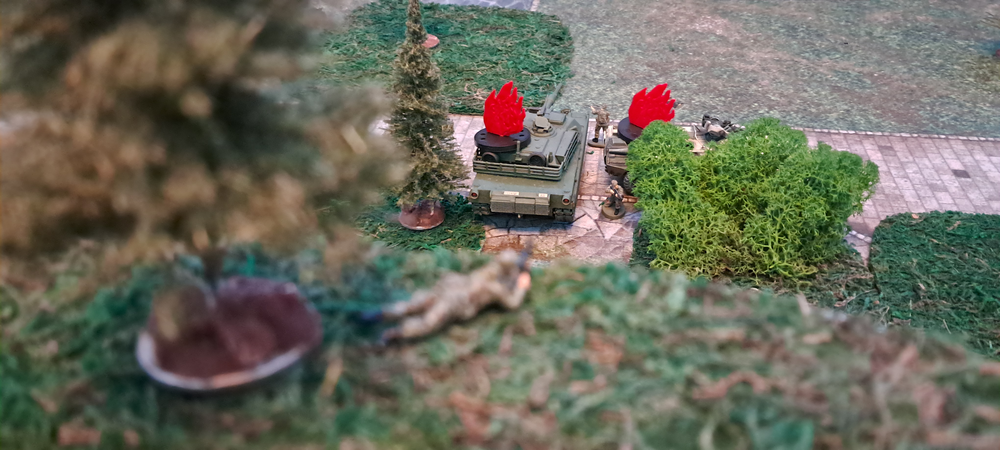
\includegraphics[width=\linewidth]{media/contract/image19.png}

Снайперские винтовки создаются специально для ведения огня на длинные
расстояния и не предназначаются для ведения ближнего боя.

В их конструкцию изначально закладывается модификатор стационарного
положения +4, но идеальная дальность для них отсутствует, таким образом
на идеальной дальности стандартный бонус +6 не применяется.

Модификатор стационарного положения самой снайперской винтовки
суммируется с модификаторами от дополнений типа сошек и оптических
прицелов. На снайперских винтовках обычно всегда имеются сошки и
оптический прицел от 10x, таким образом модификатор стационарного
положения может быть даже +9.

При стрельбе из снайперского оружия стрелок может самостоятельно выбрать
поражённых персонажей при успехе.

Стрельба из тяжёлых снайперских винтовок требует стационарного положения
(подготовки в течение 1 хода или 30 секунд). Стрельба из лёгких
снайперских винтовок возможна без подготовки, но по факту неэффективна.

\setlength\rotheadsize{3.8cm}
\begin{minipage}{\columnwidth}
\small
\begin{talltblr}[
  caption = {Характеристики снайперских винтовок},
  label = {table-sniper-rifles}
]{
  hlines,
  row{odd}={fg=navy},
  row{even}={fg=black},
  colspec={ Q[c,m,co=3]Q[c,m,co=1]Q[c,m,co=1]Q[c,m,co=1]Q[c,m,co=1]Q[c,m,co=1]Q[c,m,co=1]Q[c,m,co=1]Q[c,m,co=1] },
}
Название & \rothead{Вес, кг} & \rothead{Вес\\боеприпасов, кг} & \rothead{Максимальная\\дальность, см} & \rothead{Бронебойность (\textbf{ББ})} & \rothead{Интенсивность\\огня (\textbf{ИО})} & \rothead{Прицел} & \rothead{Только стационарное\\положение} & \rothead{Модификатор\\стационарного положения} \\
\SetRow{font=\footnotesize}H\&K G28 & 5.7 & 0.1 & 80 & 1 & 1 & 10x & $-$ & +8 \\
\SetRow{font=\footnotesize}СВЧ-308 7,62 & 5.3 & 0.1 & 120 & 1 & 1 & 12x & $-$ & +8 \\
\SetRow{font=\footnotesize}Barret M107A1 & 13.7 & 0.2 & 150 & 3 & 1 & 30x & + & +9 \\
\end{talltblr}
\end{minipage}

\subsubsection{Модификации стрелкового оружия}\label{weapon-mods}

На стрелковое оружие можно установить различные приспособления.
Существенно они не меняют показатели вооружения, но, всё же, могут
давать некоторые преимущества.

Лазерные прицелы видимого спектра устанавливаются на пистолеты и
увеличивают идеальную дальность стрельбы до 2 см.

Лазерные прицелы ИК спектра устанавливаются на пистолеты,
пистолеты-пулемёты, штурмовые винтовки и увеличивают идеальную дальность
стрельбы на 20\% с округлением вверх, но этот бонус доступен только при
использовании ПНВ.

Коллиматорные прицелы устанавливается на пистолеты, пистолеты-пулемёты и
штурмовые винтовки и увеличивают идеальную дальность стрельбы на 30\% с
округлением вверх.

Оптические прицелы устанавливаются на снайперские винтовки и другое
оружие и увеличивают модификатор стационарного положения в зависимости
от кратности, а также позволяют вести наблюдение\footnote{См. стр.~\pageref{observation}, \ref{observation}~\nameref{observation}.},
однако у оптических прицелов обычно меньше угол
обзора, чем у бинокля, поэтому их оптические характеристики несколько
ниже \footnote{См. стр.~\pageref{observation}, \ref{observation}~\nameref{observation} и Таблицу~\ref{table-visibility-equipment}.}

\setlength\rotheadsize{3cm}
\begin{minipage}{\columnwidth}
\begin{talltblr}[
  caption = {Характеристики оптических прицелов},
  label = {table-optics},
  note{1}={\footnotesize См. стр.~\pageref{mod-stationary}, \ref{mod-stationary}~\nameref{mod-stationary}.}
]{
  hlines,
  row{odd}={fg=navy},
  row{even}={fg=black},
  colspec={ Q[c,m, co=1] Q[c,m, co=1] Q[c,m, co=3] },
}
\SetRow{font=\footnotesize}Кратность & Модификатор стационарного положения\TblrNote{1} & Оптические характеристики (модификатор днём/в сумерки/макс. дальность, см) \\
2x--4x & +1 & $-$ / $-$ / 200 \\
5x--8x & +2 & +2 / $-$ / 240 \\
9x--23x & +3 & +3 / +1 / 280 \\
24x--32x & +4 & +4 / +2 / 320 \\
\end{talltblr}
\end{minipage}

Приборы ночного видения и тепловизоры можно использовать только
совместно с коллиматорами, лазерными прицелами и открытыми прицельными
приспособлениями, но нельзя использовать с оптическими прицелами.

Оптические прицелы ночного видения и прицелы с тепловизорами,
устанавливаемые на оружие, имеют такие же модификаторы и дальности как
приборы соответствующие приборы наблюдения\footnote{См. стр.~\pageref{table-visibility-equipment}, \autoref{table-visibility-equipment}~\nameref{table-visibility-equipment}.}

Сошки устанавливаются на пулемёты и снайперские винтовки и дают оружию
модификатор стационарного положения +1.

Модификатор стационарного положения для сошек и прицелов суммируется.

Приборы бесшумной стрельбы (глушители, звукоподавители) устанавливаются
на пистолеты, пистолеты-пулемёты, штурмовые и снайперские винтовки и
отменяют автоматическую демаскировку при стрельбе, сокращая при этом
эффективную и максимальную дистанции на 20\%. Для пистолета дальности не
меняются.

\paragraph{Пример}\label{example-endurance-5}

Снайперская винтовка СВЧ-308 с сошками и оптическим прицелом кратностью
12x будет иметь идеальную дальность 0 (нет огня очередями), эффективную
дальность 80, максимальную дальность 80, возможность наблюдения днём с
модификатором видимости +3 с максимальной дальностью 280 и модификатором
стационарного положения +9.

\subsubsection{Дроны}\label{drones}

Дроны --- это малые Беспилотные Летательные Аппараты (БПЛА), запускаемые
и управляемые оператором.

Все беспилотные летательные аппараты требуют сохранения стационарного
положения запускающего персонажа в процессе работы. При потере
стационарного положения управляющего персонажа БПЛА разрушается.

Все дроны позволяют осуществлять наблюдение\footnote{См. стр.~\pageref{observation}, \ref{observation}~\nameref{observation}.} с воздуха в радиусе своей скорости при отсутствии
линии видимости до цели. При успешном обнаружении цель остаётся
обнаруженной, пока находится в радиусе скорости дрона от его текущего
положения.

Разведывательный дрон не имеет вооружения.

Дрон с гранатой -- это разведывательный дрон, способный осуществить
сброс гранаты на цель сверху. После этого он продолжает работать как
обычный разведывательный дрон. Персонаж, обладающий навыком ЭЛ может
переделать разведывательный дрон в дрон с возможностью сброса (проверка
ЭЛ со сложностью 20, при неудаче дрон перестаёт функционировать; ремонт
дрона -- проверка ЭЛ со сложностью 20, при неудаче дрон превращается в
запчасти для дрона, с помощью которых можно снизить сложность ремонта
других дронов). На дрон со сбросом можно подвешивать одну любую гранату.
Прицеливание и сброс занимают весь ход (30 секунд).

Ударные дроны, также называемые барражирующими боеприпасами, тоже
способны осуществлять наблюдение, а также способны атаковать цель, но
при этом они разрушаются.

В любом случае, атака выполняется с использованием навыка ДРН в радиусе
скорости дрона от его текущего положения.

Обычно дроны используют радиоканал связи, поэтому не могут обнаружить
людей и технику под крышей в здании, но бывают также дроны на
оптоволоконном канале, и тогда у них нет ограничений.

При атаке барражирующим боеприпасом атакованный пехотный отряд может
защититься от такой атаки, если хотя бы у одного из солдат в этом отряде
есть дробовик, при этом расходуется его боезапас.

\setlength\rotheadsize{2.9cm}
\begin{minipage}{\columnwidth}
\begin{talltblr}[
  caption = {Характеристики беспилотных летательных аппаратов},
  label = {table-drones}
]{
  hlines,
  row{odd}={fg=navy},
  row{even}={fg=black},
  colspec={ Q[c,m,co=4]Q[c,m,co=1]Q[c,m,co=1]Q[c,m,co=1]Q[c,m,co=1]Q[c,m,co=1] },
}
 & \rothead{Вес, кг} & \rothead{Скорость, см} & \rothead{Количество\\ходов в игре} & \rothead{Бронебойность (ББ)} & \rothead{Интенсивность\\огня (ИО)} \\
\SetCell{font=\footnotesize}{Разведывательный дрон} & 2 & 50 & 50 & $-$ & $-$ \\
\SetCell{font=\footnotesize}{Дрон со сбросом} & 3 & 50 & 30 & 2 & 2 \\
\SetCell{font=\footnotesize}{Ударный дрон c радиоканалом} & 12 & 60 & 40 & 8 & 3 \\
\SetCell{font=\footnotesize}{Ударный дрон с оптоволоконным каналом} & 12 & 60 & 40 & 8 & 3 \\
\end{talltblr}
\end{minipage}

\subsubsection{Взрывные устройства и мины}\label{explosives-mines}

Пластичные взрывчатые вещества (например, C-4 или пластит) обычно бывают
в брикетах по ½ кг или по 1 кг. Эти вещества стабильны и безопасны, они
не взрываются из-за механического воздействия. Для взрыва используются
различные детонаторы:

\begin{itemize}
\item
  таймер, который можно установить на определённое время;
\item
  радиоприёмник, способный принять сигнал на расстоянии до 300 см;
\item
  различные датчики, которые срабатывают при приближении целей ---
  используются в минах.
\end{itemize}

В противопехотных минах взрывчатка комбинируется с поражающими
элементами, например, металлическими шариками, что увеличивает радиус
поражения.

Противопехотные мины типа ПФМ или Dragontooth не предназначены для
установки вручную, такие минные поля создаются сбросом кассет с
самолётов или ракет. При этом образуется минное поле, где мина будет
срабатывать при передвижении пехотных отрядов каждый 1 см.

В современных противотанковых минах, таких как ТМК, используются
специальные металлические формы, в которые помещается взрывчатка, для
создания направленной кумулятивной струи.

К взрывчатке и минам можно подключать дополнительные детонаторы, чтобы
обеспечить дистанционный или отложенный подрыв.

При установке мины сохраняются очки тренированности навыков МСК и ВЗР
устанавливающего её персонажа (для дистанционного минирование эти
значение всегда 0 и 1 соответственно).

Отряд пехоты способен обнаружить мины и взрывные устройства при
передвижении, если не используется бег. Когда отряд проходит в пределах
1 см от мины или минного поля, он обнаруживает мину автоматически. При
этом отряд останавливается и необходимо сделать бросок на
наблюдение\footnote{См. стр. \pageref{observation}, \ref{observation} \nameref{observation}.} Если бросок успешен, то отряд обнаруживает мину.
Если бросок неуспешен, то отряд подрывается на мине.

Мины и взрывные устройства может обезвредить персонаж с ненулевым
навыком ВЗР. Сложность рассчитывается как удвоенный ВЗР минёра минус
удвоенный ВЗР сапёра. Для успешного обезвреживания нужно выбросить на
кубике D20 значение больше получившейся сложности. Это значит, что
делать бросок имеет смысл только если ВЗР сапёра меньше ВЗР минёра.

При взрыве устройства расчёт эффекта применяется как при стрельбе. При
этом применяется модификатор навыка (используется сохранённое значение
ВЗР для взрывного устройства). Всегда применяется модификатор флангового
огня, и для пехоты, и для техники. Остальные модификаторы не
применяются.

При использовании взрывных устройств в помещении показатель
интенсивности огня удваивается.

\setlength\rotheadsize{2.9cm}
\begin{minipage}{\columnwidth}
\begin{talltblr}[
  caption = {Характеристики взрывных устройств и мин},
  label = {table-explosives},
  note{1}={\footnotesize Для поражения пехоты требует установки дополнительного детонатора, т.к. встроенный срабатывает только на технику.}
]{
  hlines,
  row{odd}={fg=navy},
  row{even}={fg=black},
  colspec={ Q[c,m,co=6] Q[c,m,co=1] Q[c,m,co=1] Q[c,m,co=1] },
}
 & Вес, кг & \rothead{Бронебойность (ББ)} & \rothead{Интенсивность\\огня (ИО)} \\
Противопехотная мина ПФМ & $-$ & $-$ & 1 \\
Противопехотная мина ОЗМ & 5 & $-$ & 4 \\
Противотанковая мина ТМ & 11 & 6 & 4\TblrNote{1} \\
Противотанковая мина ТМК & 11.5 & 10 & 2 \\
Взрывчатка & 1 & 1 & 1 \\
Взрывчатка & 2 & 2 & 2 \\
Взрывчатка & 3 & 3 & 2 \\
Взрывчатка & 5 & 4 & 3 \\
Взрывчатка & 10 & 6 & 4 \\
\end{talltblr}
\end{minipage}

\end{multicols}
\clearpage
\begingroup
\footnotesize

\subsection{Вооружение техники}\label{vehicle-weapons}

\setlength\rotheadsize{3cm}
\begin{minipage}{\columnwidth}
\begin{talltblr}[
  caption = {Характеристики вооружения техники},
  label = {table-vehicle-weapons},
  note{1}={\footnotesize Свойства оружия:\\С --- только стрельба из стационарного положения.\\В --- возможна стрельба по воздушным целям.\\А--- стрельба непрямой наводкой.}
]{
  hlines,
  row{odd}={fg=navy},
  row{even}={fg=black},
  colspec={Q[l,m,co=7]Q[c,m,co=1]Q[c,m,co=1]Q[c,m,co=1]Q[c,m,co=1]Q[c,m,co=1]Q[c,m,co=1]Q[c,m,co=1]Q[c,m,co=1]},
}
Название & \rothead{Идеальная\\дальность, см} & \rothead{Эффективная\\дальность, см} & \rothead{Максимальная\\дальность, см} & \rothead{Радиус\\отклонения, см} & \rothead{Бронебойность (\textbf{ББ})} & \rothead{Интенсивность\\огня (\textbf{ИО})} & \rothead{Осколочно-фугасное\\действие (\textbf{ОФ})} & \rothead{Свойства\TblrNote{1}} \\
\SetCell[c=9]{c}{Пулемёты} \\
Пулемёт & 40 & 80 & 160 & $-$ & 2 & 3 & $-$ & В \\
Крупнокалиберный пулемёт 12,7--14,5 мм & 50 & 100 & 200 & - & 3 & 3 & $-$ & В \\
\SetCell[c=9]{c}{Автоматические пушки} \\
Автоматическая пушка 20 мм & 50 & 100 & 200 & $-$ & 4 & 3 & $-$ & В \\
Автоматическая пушка 30 мм & 50 & 100 & 200 & $-$ & 6 & 3 & $-$ & В \\
Автоматическая пушка 40, 57 мм & 50 & 100 & 200 & $-$ & 7 & 3 & $-$ & В \\
\SetCell[c=9]{c}{Реактивные гранатомёты} \\
Безоткатное орудие 73 мм & 40 & 80 & 160 & $-$ & 8 & 3 & $-$ & $-$ \\
\SetCell[c=9]{c}{ПТРК} \\
MILAN & 240 & 240 & 240 & $-$ & 10 & $-$ & $-$ & С \\
\SetCell[c=9]{c}{Танковые орудия} \\
Танковое орудие 125 мм & 60 & 120 & 240 & $-$ & 11 & 4 & $-$ & $-$ \\
\SetCell[c=9]{c}{Артиллерийские системы} \\
Гаубица 122 мм & $-$ & $-$ & 1000 & 5 & 8 & 4 & $-$ & СА \\
Гаубица 155 мм & $-$ & $-$ & 2000 & 6 & 8 & 4 & $-$ & СА \\
\SetCell[c=9]{c}{Ракетные системы залпового огня} \\
РСЗО 122 мм & $-$ & $-$ & 1200 & 15 & 8 & 4 & $-$ & СА \\
\end{talltblr}
\end{minipage}

\subsection{Бронебойность и бронированность}\label{armor}

\begin{minipage}{\columnwidth}
\begin{talltblr}[
  caption = {Бронебойность оружия (ББ) и броня техники (Бр)},
  label = {table-armor},
  note{1}={\footnotesize ОФ --- Осколочно-Фугасные гранаты, мины, снаряды.},
  note{2}={\footnotesize БП --- Бронебойные Пули.},
  note{3}={\footnotesize БС --- кинетический Бронебойный Снаряд, в том числе, например, БОПС --- Бронебойный Оперённый Подкалиберный Снаряд.},
  note{4}={\footnotesize БК --- Бронебойный Кумулятивный боеприпас (снаряд, ракета, мина).}
]{
  hlines,
  row{odd}={fg=navy},
  row{even}={fg=black},
  colspec={ Q[c,m,co=1] Q[c,m,co=7] Q[c,m,co=1] Q[c,m,co=1] Q[c,m,co=1] Q[c,m,co=1] Q[c,m,co=1] Q[c,m,co=1] Q[c,m,co=1] Q[c,m,co=1] Q[c,m,co=1] Q[c,m,co=1] Q[c,m,co=1] },
}
\SetCell[r=3]{c} Броня (\textbf{Бр}) & \SetCell[r=3]{c} {} & \SetCell[c=11]{c} Бронебойность оружия (\textbf{ББ}) & & & & & & & & & & \\
& & \SetCell[c=3]{c} ОФ\TblrNote{1}, БП\TblrNote{2} & & & \SetCell[c=4]{c} БС\TblrNote{3} автопушек, ОФ мины & & & & \SetCell[c=4]{c} БС большого калибра, БК\TblrNote{4} & & & \\
& & 1 & 2 & 3 & 4 & 5 & 6 & 7 & 8 & 9 & 10 & 11 \\
0 & Небронированная & & & & & & & & & & & \\
& Уничтожена & 20+ & 14+ & 11+ & 8+ & 7+ & 7+ & 7+ & 7+ & 7+ & 7+ & 7+ \\
& Стресс & 13+ & 8+ & 5+ & 3+ & 3+ & 4+ & 5+ & & & & \\
2 & Легкобронированная & & & & & & & & & & & \\
& Уничтожена & & & 19+ & 18+ & 15+ & 14+ & 13+ & 11+ & 10+ & 8+ & 7+ \\
& Стресс & & & 13+ & 12+ & 11+ & 10+ & 9+ & 9+ & 8+ & 6+ & \\
4 & Тяж. бронированная & & & & & & & & & & & \\
& Уничтожена & & & & & 21+ & 19+ & 17+ & 15+ & 13+ & 11+ & 9+ \\
& Стресс & & & & & 16+ & 14+ & 12+ & 13+ & 11+ & 9+ & 7+ \\
5 & Танк 1 поколения & & & & & & & & & & & \\
& Уничтожен & & & & & & 24+ & 22+ & 20+ & 19+ & 17+ & 15+ \\
& Стресс & & & & & & 20+ & 18+ & 18+ & 17+ & 15+ & 13+ \\
6 & Танк 2 поколения & & & & & & & & & & & \\
& Уничтожен & & & & & & & 25+ & 23+ & 21+ & 19+ & 17+ \\
& Стресс & & & & & & & 21+ & 20+ & 19+ & 17+ & 15+ \\
7 & Танк 3 поколения & & & & & & & & & & & \\
& Уничтожен & & & & & & & & 26+ & 23+ & 21+ & 19+ \\
& Стресс & & & & & & & & 23+ & 21+ & 19+ & 17+ \\
\end{talltblr}
\end{minipage}

\clearpage
\endgroup

\begin{multicols}{2}
\raggedcolumns{}

\subsection{Огневая поддержка}\label{fire-support-section}

Огневая поддержка --- это навесная стрельба или стрельба непрямой
наводкой.

Для гранат, подствольных и автоматических гранатомётов, миномётов,
гаубиц, систем залпового огня и тактических ракет не обязательно наличие
линии видимости.

Стрельба непрямой наводкой, кроме ручных гранат, требует стационарного
положения боевой единицы.

\subsubsection{Гранаты}\label{grenades-section}

Гранаты можно метать без наличия линии видимости, например, перекидывать
через высокий забор. Это не требует пристрелки и корректировки.

\subsubsection{Гранатомёты}\label{grenade-launchers}

Стрельба из гранатомётов при отсутствии линии видимости требует
пристрелки и корректировки.

\subsubsection{Ствольная артиллерия и миномёты}\label{artillery-mortars}

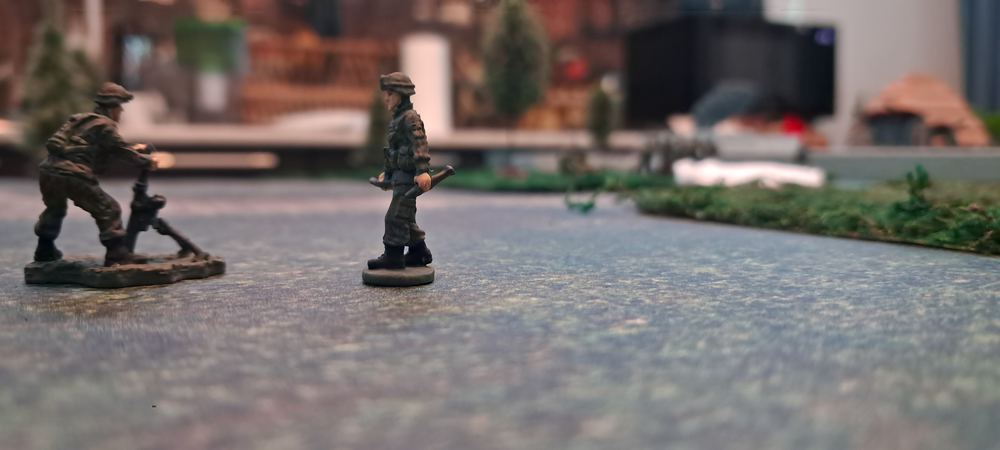
\includegraphics[width=\linewidth]{media/contract/image20.png}

Стрельба из ствольной артиллерии может вестись корректируемыми или
обычными боеприпасами.

Стрельба корректируемыми боеприпасами ведётся по обычным правилам и не
требует пристрелки\footnote{См. стр. \pageref{hit-effects}, \ref{hit-effects} \nameref{hit-effects}.}, но не может вестись «по карте», без
корректировки.

Стрельба обычными боеприпасами требует пристрелки и корректировки, а
также может вестись «по карте», без корректировки. Такой огонь может
вестись только по определённому ориентиру: перекрёстку, дому, мосту. В
этом случае применяется модификатор огня вслепую\footnote{См. стр. \pageref{mod-blind}, \ref{mod-blind} \nameref{mod-blind}.},
а очки корректировки всегда считаются равными 0 независимо от того, сколько выстрелов делалось в одну и ту же точку.

\subsubsection{Ракетные системы залпового огня}\label{mlrs}

РСЗО не требуют пристрелки. При выстреле для всех боевых единиц
противника в радиусе отклонения можно отдельно провести расчёт эффектов
от попадания по обычной схеме.

\subsubsection{Пристрелка}\label{ranging}

Изначально при стрельбе по какой-либо цели орудие имеет 0 очков
корректировки. Каждый последовательный выстрел этого орудия по той же
цели увеличивает очки корректировки этого орудия на 1, при условии, что
цель демаскирована на момент выстрела (корректировщик наблюдает цель).

Очки корректировки уменьшаются при необходимости перенести огонь: как
минимум на 1 плюс ещё на 1 очко за каждые полные 10 см переноса.

Очки корректировки сбрасываются на 0, если орудие теряет стационарное
положение, сдвигается или переключается на огонь вслепую.

Максимально у орудия может быть 5 очков корректировки.

При выстреле по цели производится бросок кубика D20, к результату
применяется модификатор навыка\footnote{См. стр. \pageref{mod-skill}, \ref{mod-skill} \nameref{mod-skill}.} Ур(X) и оценивается по таблице исходя
из текущих очков корректировки орудия (см. \autoref{table-fire-correction}).

\begin{center}
\begin{minipage}{0.7\columnwidth}
\begin{talltblr}[
  caption = {Пристрелка и корректировка при стрельбе непрямой наводкой},
  label = {table-fire-correction}
]{
  hlines,
  row{odd}={fg=navy},
  row{even}={fg=black},
  colspec={ Q[c,m,co=1] Q[c,m,co=1] },
}
Очки корректировки & Результат с учётом навыка \\
0 & 22+ \\
1 & 19+ \\
2 & 14+ \\
3 & 8+ \\
4 & 4+ \\
5 & 1+ \\
\end{talltblr}
\end{minipage}
\end{center}

В случае успеха тот же самый результат кубика снова используется для
определения эффекта от попадания по цели.

Если пехотные отряды стоят вплотную друг к другу (например, происходит
штурм), то они все считаются поражёнными, к каждому следует применить
эффект от попадания отдельно.

В случае промаха, если в радиусе, определяемом как
(5~--~Очки\textsubscript{Корректировки})~×~Радиус\textsubscript{Отклонения},
есть другие отряды, то нужно последовательно провести дополнительную
проверку на попадание по каждому из них с такими же параметрами, что по
искомой цели, до получения первого попадания.

\subsubsection{Эффекты от попадания}\label{hit-effects}

Эффекты от попадания определяются как при обычной стрельбе: используется
результат броска кубика, применяются модификаторы при стрельбе, а также
показатель интенсивности огня орудия.

При попадании непрямой наводкой всегда применяется модификатор
флангового огня\footnote{См. стр.~\pageref{mod-flank}, \ref{mod-flank}~\nameref{mod-flank}.} Если укрытие не защищает боевую единицу со всех сторон, то
модификатор укрытия не применяется.

\subsection[Радиосвязь и РЭБ]{\texorpdfstring{Радиосвязь и РЭБ\footnote{РадиоЭлектронная Борьба}}{Радиосвязь и РЭБ}}\label{radio-ew}

Персонажи могут общаться знаками или голосом в пределах одного отряда
или между отрядами на дистанции до 4 см. Для передачи данных и команд на
большие расстояния используется радиосвязь. Радиосвязь необходима для
корректировки огня артиллерии, передачи информации о демаскированных
боевых единицах другим отрядам, управления дронами с радиоканалом,
дистанционного подрыва мин.

Сотовые телефоны работают не везде, но там, где работают, позволяют
связаться на любое расстояние посредством сети базовых станций.
Переносные и возимые радиостанции позволяют не зависеть от
инфраструктуры. Радиостанции могут работать как ретрансляторы, позволяя
увеличивать зону устойчивой связи, а размещение радиостанции на высоте
позволяет вдвое увеличить дальность её действия. Наконец, терминал
спутниковой связи позволяет выходить на связь с другим обладателем
терминала на любом расстоянии. Терминалы спутниковой связи требуют
настройки и стационарного положения во время использования.

Радиостанции могут быть трёх уровней защищённости: 1 уровень соответствует сотовой связи,
гражданским и устаревшим военным радиостанциям, 2 и 3 уровни соответствуют военным радиостанциям 5 и 6 поколения
соответственно.

\setlength\rotheadsize{1.5cm}
\begin{minipage}{\columnwidth}
\small
\begin{talltblr}[
  caption = {Переносные средства связи},
  label = {table-portable-comms}
]{
  hlines,
  row{odd}={fg=navy},
  row{even}={fg=black},
  colspec={ Q[c,m,co=2]Q[c,m,co=1]Q[c,m,co=1]Q[c,m,co=4]Q[c,m,co=3] },
}
Тип & \rothead{Уровень} & \rothead{Вес, кг} & Название & Радиус передачи, см \\
Сотовый & 1 & 0.5 & {Apple\\Samsung} & $\infty$ (в зоне покрытия) \\
Радио & 1 & 0.5 & Baofeng Motorola & 200 \\
Радио & 2 & 1.0 & Р-168 Акведук & 200 \\
Радио & 3 & 0.5 & Р-187-П1 Азарт & 200 \\
Спутник & 2 & 16.0 & Р-438М Белозер & $\infty$ \\
\end{talltblr}
\end{minipage}

\setlength\rotheadsize{1.5cm}
\begin{minipage}{\columnwidth}
\begin{talltblr}[
  caption = {Возимые средства связи},
  label = {table-vehicle-comms}
]{
  hlines,
  row{odd}={fg=navy},
  row{even}={fg=black},
  colspec={ Q[c,m,co=2] Q[c,m,co=1] Q[c,m,co=5] Q[c,m,co=2] },
}
Тип & \rothead{Уровень} & Название & Радиус передачи, км \\
Радио & 2 & Р-168-100У Акведук & 200 \\
Радио & 3 & Р-187ВЕ Азарт & 200 \\
Спутник & 2 & Р-448 Аурига & $\infty$ \\
\end{talltblr}
\end{minipage}

Для подавления радиосвязи, в том числе для выведения из строя дронов с
радиоканалом управления, существуют станции РЭП\footnote{РадиоЭлектронное Подавление}.
Станции РЭП могут быть 1 или 2 уровней и подавлять радиостанции того же или меньшего уровня.
Станции РЭП могут подавить разведывательные дроны, дроны со сбросом, а также барражирующие
боеприпасы с радиоканалом. Все дроны и пульты управления ими считаются средствами радиосвязи 4 уровня.

\setlength\rotheadsize{1.5cm}
\begin{minipage}{\columnwidth}
\begin{talltblr}[
  caption = {Переносные средства РЭП},
  label = {table-portable-ew}
]{
  hlines,
  row{odd}={fg=navy},
  row{even}={fg=black},
  colspec={ Q[c,m,co=1]Q[c,m,co=1] Q[c,m,co=5] Q[c,m,co=3] },
}
\rothead{Уровень} & \rothead{Вес, кг} & Название & Радиус подавления, см \\
1 & 3.8 & Капюшон & 20 \\
2 & 20.0 & Гарпия Периметр & 60 \\
\end{talltblr}
\end{minipage}

\setlength\rotheadsize{1.5cm}
\begin{minipage}{\columnwidth}
\begin{talltblr}[
  caption = {Возимые и стационарные средства РЭП},
  label = {table-vehicle-ew}
]{
  hlines,
  row{odd}={fg=navy},
  row{even}={fg=black},
  colspec={ Q[c,m,co=1] Q[c,m,co=5] Q[c,m,co=3] },
}
\rothead{Уровень} & Название & Радиус подавления, см \\
1 & Капюшон & 40 \\
2 & Ромашка & 100 \\
2 & Чистюля & 300 \\
\end{talltblr}
\end{minipage}

Отряды, попадающие в зону действия РЭП, не могут корректировать огонь
артиллерии, не могут управлять дронами, не могут дистанционно подрывать
мины, не могут передавать информацию другим отрядам и принимать
информацию. Дроны на радиоуправлении, попавшие в зону действия РЭП,
немедленно выходят из строя. Мины с радиовзрывателем, попавшие в зону
действия РЭП, не срабатывают.

Если отряд без связи демаскирует вражескую боевую единицу, он делает это
только в рамках своего действия (например, другие персонажи отряда могут
вести огонь без модификатора огня вслепую), но фактически состояние
маскировки сохраняется.

Помимо РЭП, существуют станции РЭР\footnote{РадиоЭлектронная Разведка},
предназначенные для анализа радиосигналов противника. Они позволяют
перехватывать и подделывать сообщения. Станции РЭР могут быть 1, 2 и 3 уровней.

\begin{minipage}{\columnwidth}
\begin{talltblr}[
  caption = {Возимые и стационарные средства РЭР},
  label = {table-vehicle-esm}
]{
  hlines,
  row{odd}={fg=navy},
  row{even}={fg=black},
  colspec={Q[c,m,co=1] Q[c,m,co=4]Q[c,m,co=2] Q[c,m,co=2] },
}
Уровень & Название & Радиус подавления, см & Радиус передачи, км \\
1 & Леер & 100 & 200 \\
2 & Беркут & 200 & 200 \\
3 & Монолит & 300 & 200 \\
\end{talltblr}
\end{minipage}

Любые боевые единицы, использующие радиосвязь, регистрируемую РЭР,
демаскируются, в том числе и другие станции РЭР, которые передают
сообщения, а не только принимают, и станции РЭП того же уровня или
уровнем ниже. Если отряд находится за пределами игровой области,
считается, что известны его точные координаты, которые можно
использовать, например, для возможности организации артиллерийского
удара.

Отряд, использующий станцию РЭР получает возможность попытаться отдать
фальшивую команду любому вражескому отряду или дрону, находящемуся в
радиусе действия станции РЭР.

При отдаче команды вражескому отряду этом необходимо пройти состязание с
использованием навыка ЛИД с командиром вражеского отряда. В случае
успеха, в следующий ход он будет обязан попытаться выполнить эту команду.

При отдаче команды вражескому дрону дополнительных проверок не требуется.

РЭР может перехватывать и подделывать сообщения радиостанций такого же
уровня и ниже, даже если те находятся в зоне действия РЭП того же или
более низкого уровня. Однако РЭР не может работать в зоне РЭП более
высокого уровня.

Получение радиостанции, настроенной на частоту других отрядов, позволяет
до изменения частоты этими отрядами выполнять те же самые действия, что и РЭР:
отдавать фальшивые команды и вести переговоры от лица предыдущего владельца радиостанции.

Иерархия взаимодействия на одном уровне: радиостанция~\textless~РЭП~\textless~РЭР.
Это означает, что РЭП подавляет радиостанции того же уровня и ниже, но РЭР того же уровня может работать поверх РЭП того же уровня.
Станция РЭР может работать как радиостанция или как станция РЭП того же радиуса и такого же уровня.

Для определения координат артиллерии существуют станции радиолокационной
разведки. Такие станции могут определять координаты артиллерии и
миномётов, ведущих огонь, для нанесения по ним артиллерийского удара.
Кроме того, они могут обнаруживать боевые единицы в радиусе своего
действия независимо от времени суток и погодных условий. Станция
радиолокационной разведки неуязвима к РЭП.

\begin{minipage}{\columnwidth}
\begin{talltblr}[
  caption = {Переносные РЛС},
  label = {table-portable-radar}
]{
  hlines,
  row{odd}={fg=navy},
  row{even}={fg=black},
  colspec={Q[c,m,co=3]Q[c,m,co=1]Q[c,m,co=1]},
}
Название & Вес, кг & Радиус, см \\
Соболятник & 36.0 & 600 \\
\end{talltblr}
\end{minipage}

\begin{minipage}{\columnwidth}
\begin{talltblr}[
  caption = {Возимые РЛС},
  label = {table-vehicle-radar}
]{
  hlines,
  row{odd}={fg=navy},
  row{even}={fg=black},
  colspec={Q[c,m,co=3]Q[c,m,co=1]Q[c,m,co=1]},
}
Название & Радиус, см \\
Зоопарк & 3000 \\
AN/TPQ-53 & 3000 \\
\end{talltblr}
\end{minipage}

\end{multicols}

\end{document}
